\listfiles
\documentclass[12pt]{report}  %%% Changed from 12pt. Fixed dimensions
                              %%% have not been updated
%%%%
%%nomenclature hack from http://www.freiheitsfreund.de/2010/10/24/automatically-run-makeindex-from-within-a-latex-document-with-write18/%%%

\usepackage[intoc]{nomencl}

\textwidth=6in \oddsidemargin=0.2in \topmargin=-0.5in
\textheight=9in  % 9in must include page numbers
\textfloatsep = 0.4in \addtocontents{toc}{\vspace{0.4in} \hfill
Page\endgraf} \addtocontents{lof}{\vspace{0.2in} \hspace{0.13in} \
Figure\hfill Page\endgraf} \addtocontents{lot}{\vspace{0.2in}
\hspace{0.13in} \ Table\hfill Page\endgraf}

\usepackage{textcomp}
\usepackage{array}
\usepackage{listings}
\usepackage{setspace}
\usepackage{mathptmx}
\usepackage[table, svgnames]{xcolor}
\usepackage{colortbl}
\usepackage{graphicx}
\usepackage{amssymb, amsmath}
\usepackage{subfig}
\usepackage{epsfig}
\usepackage{times}
\usepackage{float}
\usepackage{rotating}
\usepackage{makeidx}
\usepackage{url}
\usepackage{multirow}
\usepackage{booktabs}
\usepackage[subfigure, titles]{tocloft}
\usepackage{acronym}
\usepackage{datetime}
\usepackage{gensymb}
\usepackage{epigraph}



%%another algorithm package
\usepackage{algorithm}
\usepackage{algorithmic}

\renewcommand{\nomname}{LIST OF ABBREVIATIONS}
\makenomenclature

% New command: caption for name
\newcommand\tline[2]{$\underset{\text{#1}}{\text{\underline{\hspace{#2}}}}$}

% New command: change margin for dedication
\def\changemargin#1#2{\list{}{\rightmargin#2\leftmargin#1}\item[]}
\let\endchangemargin=\endlist 

\graphicspath{{images/}}
\DeclareGraphicsExtensions{.pdf, .jpeg, .png, .PNG, .jpg, .eps, .tiff}

\urlstyle{same}

\usepackage{makecell}
\usepackage{titletoc}
\usepackage{style/sfchap}
\usepackage{style/sfsection}
\usepackage[authoryear]{natbib}
%\usepackage{apacite}
\usepackage{appendix}
%\usepackage{tocbibind}
\usepackage{tabularx}
\usepackage[nottoc]{tocbibind}

% Default counter is 7, change to 1 for only sections
\setcounter{secnumdepth}{1}
\setcounter{tocdepth}{1}

\usepackage{hyperref}
\hypersetup{
	pdftitle={Attributes of Brain Functional Network Architecture Supporting Skilled Reading},
	pdfauthor={Stephen Bailey},
	bookmarksnumbered, %Determined if chapter numbers are included in the bookmark list
	pdfstartview={FitH},
	pdfborder={0 0 0},
	plainpages=false
}%
\usepackage[all]{hypcap}

% Stats table label
\newcommand{\statslabel}[2]{\multirowcell{#1}[-1.6mm][c]{#2}}

% Below heading rule.
\newcommand{\otoprule}{\midrule[\heavyrulewidth]}

% Prevent double spaced equations
\newenvironment{tightequation}{\singlespace\begin{equation}}{\end{equation}}

% Extra junk to pretty up the table of contents
\setlength{\cftsecnumwidth}{2.8em}
\setlength{\cftsubsecnumwidth}{3.7em}
\setlength{\cftsubsubsecnumwidth}{4.6em}
\setlength{\cftparanumwidth}{5.5em}
\setlength{\cftsubparanumwidth}{6.5em}
\setlength{\cfttabnumwidth}{3.5em}
\setlength{\cftfignumwidth}{3.5em} 

\renewcommand{\contentsname}{TABLE OF CONTENTS}
\renewcommand{\listfigurename}{LIST OF FIGURES}
\renewcommand{\listtablename}{LIST OF TABLES}
\renewcommand{\bibname}{ \texorpdfstring{{BIBLIOGRAPHY\vspace{10mm}}}{BIBLIOGRAPHY}   }
%
\renewcommand{\chaptermark}[1]{%
  \markboth{\MakeUppercase{%
      \chaptername}\ \thechapter.%
    \ #1}{}}

\newcolumntype{L}[1]{>{\raggedright\arraybackslash}p{#1}}
\newcolumntype{C}[1]{>{\centering\arraybackslash}p{#1}}
\newcolumntype{R}[1]{>{\raggedleft\arraybackslash}p{#1}}
    
\interfootnotelinepenalty=10000 %prevents the splitting of long footnotes across multiple pages. Use with caution. 

\begin{document}

%%%%%%%%%%%%%%%%%%%%%%%%%%%%%%%%%%%%%%%%%%%%%%%%%%%%%%%%%%%%%%%%%%%%%%%%%%%%%%%%
%% Prevent the warning: pdfTeX warning (ext4): destination with the same identifier (name{page.1}) has been already used, duplicate ignored
%%	This setting will make a difference to the output because the page number is suppressed for the title page
\pagenumbering{alph}

\begin{titlepage}
\thispagestyle{empty}\enlargethispage{\the\footskip}%
\begin{center}
	{\setstretch{1.66} \textsc{Attributes of Brain Functional Network Architecture\\ Supporting Skilled Reading}}\par%
	\vskip.5in
	By
	\vskip .4in
	{Stephen K. Bailey}
	\vskip .4in
	
	\begin{doublespace}
	Dissertation\\
		Submitted to the Faculty of the \\
		Graduate School of Vanderbilt University \\
		in partial fulfillment of the requirements \\
		for the degree of \\ [.2in]
	\end{doublespace}
	
	\textsc{Doctor of Philosophy} \\[.2in]
	in \\[.15in]
	\textsc{Neuroscience} \\[.25in]
	December 15, 2018 \\[0.1in]
	Nashville, Tennessee
	\vskip .5in
\end{center}
%%%Uncomment for Signatures%%%
\hspace*{0.3in} Approved: \hskip 3.4in Date:\\[1em]
% \hspace*{1.0in} \rule{3.0in}{.5pt} \hskip 0.1in \rule{1in}{.5pt} \\[.1in]
% \hspace*{1.0in} \rule{3.0in}{.5pt} \hskip 0.1in \rule{1in}{.5pt} \\[.1in]
% \hspace*{1.0in} \rule{3.0in}{.5pt} \hskip 0.1in \rule{1in}{.5pt} \\[.1in]
% \hspace*{1.0in} \rule{3.0in}{.5pt} \hskip 0.1in \rule{1in}{.5pt} %\\[.1in]

\hspace*{0.05in} \tline{Professor Adam Anderson \hspace*{2.6in}}{4.0in} \hskip 0.1in  \tline{}{1.0in} \\[.25in]
\hspace*{.3in} \tline{Professor Laurie Cutting \hspace*{2.7in}}{4.0in} \hskip 0.1in  \tline{}{1.0in} \\[.25in]
\hspace*{0.3in} \tline{Professor Zhaohua Ding \hspace*{2.71in}}{4.0in} \hskip 0.1in \tline{}{1.0in} \\[.25in]
\hspace*{0.3in} \tline{Professor Gavin Price \hspace*{2.83in}}{4.0in} \hskip 0.1in \tline{}{1.0in} 

%%%%%%%%%%%%%%
%%%%%%Uncomment  for Approved Names%%%%%%
% \begin{center}
% \begin{doublespace}
% Approved:\\
% \hspace*{1.0in} Professor Laurie Cutting \\

% Professor Adam Anderson \\
% Professor Zhaohua Ding \\
% Professor Gavin Price  \\
% \end{doublespace}
% \end{center}
\end{titlepage}

%%%%%%%%%%%%%%%%%%%%%%%%%%%%%%%%%%%%%%%%%%%%%%%%%%%%%%%%%%%%%%%%%%%%%%%%%%%%%%%%
\doublespacing
\pagenumbering{roman} \setcounter{page}{2}

%%%%%%%%%%%%%%%%%%%%%%%%%%%%%%%%%%%%%%%%%%%%%%%%%%%%%%%%%%%%%%%%%%%%%%%%%%%%%%%%
\chapter*{DEDICATION}
\addcontentsline{toc}{chapter}{DEDICATION}
\vspace{7mm}

\begin{changemargin}{1in}{1in} 
    This work -- and especially the years of learning it is built upon -- is dedicated to my parents, Dan and Janine Bailey, who taught me to learn something from everything: novels,  newspapers, comics, classes, car rides, restaurants, sports,   sermons, trivia, movies, games, work, success and failure. Thank you for making the world a place full of meaning.
\end{changemargin} 

% %%%%%%%%%%%%%%%%%%%%%%%%%%%%%%%%%%%%%%%%%%%%%%%%%%%%%%%%%%%%%%%%%%%%%%%%%%%%%%%%
\chapter*{ACKNOWLEDGMENTS}
\addcontentsline{toc}{chapter}{ACKNOWLEDGMENTS}
\vspace{7mm}

It is wrong for me to ascribe myself as the sole author of this dissertation. The work described in the following pages is the result of the efforts of dozens of people, most notably my colleagues in Vanderbilt's Education and Brain Sciences Research Laboratory and the participants who lent their time, energy and brains to each of the studies. Julie Delheimer, Lanier Sachs, Laura Barquero, Angela Emerson, Hannah Rowland and Scott Burns worked relentlessly, year upon year, to keep the operations of our busy and growing lab humming along. Their efforts insulated myself and the rest of the research team from the everyday demands of running a high-performing lab, and they made it possible for me to focus almost exclusively on my own research and training. 

I have been privileged to train at an institution rich in resources and funding. The staff at the Imaging Institute, Brain Institute, Kennedy Center and ACCRE have been wonderful colleagues. They were patient with my questions and fumblings as I attempted to play with just about every toy I could get my hands on these past five years. The National Institutes of Health has largely underwritten these experiences, through a variety of mechanisms. These include training grants (T32 MH064913, F31 HD090923), center grants (U54 HD083211), and the many research awards granted to Dr. Cutting (R01 HD044073, R01 HD067254, among others).

I am grateful for a supportive committee that gave me guidance at critical junctures and opened my eyes to a research domains I would not have otherwise seen. Dr. Gavin Price embodied for me the rigor and theoretical drive present in the best of cognitive psychology, and our conversations helped to give a pointed form to many of the ideas explored herein. (Any deviation from clarity is my own.) Dr. Adam Anderson gave me insight into the wider field of biomedical image analysis through his classes and lectures, and he also exposed me to a more programmatic approach to analysis. This move away from GUIs and toolboxes opened me up to new tools and techniques, and it has set me up to be a much more innovative scientist. Finally, my collaborations with Dr. Zhaohua Ding gave me the unique experience of watching a scientific idea evolve from its infancy to its impact, as he chased, teased out, and trumpeted the existence of the BOLD signal in white matter tissue. His tenacity impressed upon me the role grit and sheer hard work play in pushing science forward. 

To Dr. Laurie Cutting I owe a special debt. My experience as a graduate student was unusual: I had all the resources I needed, all the data I could want, all the opportunity I could ask for, from my first day as a student. Dr. Cutting has built a world-class training environment, and she gave me five years of freedom to play in it. What is most impressive to me, though, is that she has fostered a healthy, positive, and professional team culture that has persisted even as the team has turned over and grown. It has been a joy to be a part of this team. I am grateful for the gamble that Dr. Cutting took on me, a prospective student with no background in neuroscience, no experience with imaging, no knowledge of statistics or computing or special education. That I leave with all these things and more is a direct result of the guidance, opportunity and encouragement provided by Dr. Cutting.

I have made too many friends to count or acknowledge, but I will try. My cohort of graduate students -- Mackenzie Catron, Eric Wilkey, David Simon, Dylan Morrow-Jones -- were a great source of encouragement during our first years, as I was scrambling to recover the tiny amount of biochemistry I learned in college and perplexing over $t$-statistics and ANOVA designs. Later support came from my colleagues in the lab, especially Neena Hudson, Stephanie Del Tufo, Tin Nguyen, Mercedes Spencer and Laura Barquero. Then there were those who pulled me away from brains for refreshing moments: Alice Leach, Jake Benzing, Auvy Hossasin and Nausheen Karim. Finally, I must give a special acknowledgment to the very first person I met at Vanderbilt. Katherine Aboud has been a partner and friend in all of my research endeavors -- and later, parenting efforts -- as she pushed me to remember the ``story'' in all of my ``process''. It has been a privilege to study, work and converse with these fine people, and I will miss it greatly. 

The best analogy for the PhD is that of an odyssey: the destination is clear but the path is unknown and treacherous at times. For travelling with me and keeping me grounded, I am grateful for my wife, partner and best friend, Danielle. Our particular journey has been filled with classes and experiments and writing, of course. But it has also been filled with leaky houses, arduous job searches, and, most of all, children. It has only been through her conversation, support, love, and constant reminding of the important things that this odyssey has reached its happy ending.


%%%%%%%%%%%%%%%%%%%%%%%%%%%%%%%%%%%%%%%%%%%%%%%%%%%%%%%%%%%%%%%%%%%%%%%%%%%%%%%%
\singlespacing
\tableofcontents

%%%%%%%%%%%%%%%%%%%%%%%%%%%%%%%%%%%%%%%%%%%%%%%%%%%%%%%%%%%%%%%%%%%%%%%%%%%%%%%%
\begingroup
\setlength{\parskip}{1\baselineskip}
\listoftables
\newpage
\listoffigures
\newpage
\printnomenclature
\newpage
\endgroup

%%%%%%%%%%%%%%%%%%%%%%%%%%%%%%%%%%%%%%%%%%%%%%%%%%%%%%%%%%%%%%%%%%%%%%%%%%%%%%%%
\normalsize
\doublespacing
\pagenumbering{arabic}
\setcounter{page}{1}


%% Input your chapter .tex files here.
%% Each one should begin with a call to \chapter{TITLE}
\chapter{Introduction}

\epigraph{Learning to read is probably the most difficult and revolutionary thing that happens to the human brain and if you don't believe that, watch an illiterate adult try to do it.}{John Steinbeck}

\section{Overview}
Reading is a complex cognitive act. To read, individuals must precisely control visual attention, map symbols to phonological representations, extract meaning from words, update mental representations of the text, inhibit unimportant associations, and make appropriate inferences. Consequently, while the most explicit aim of reading instruction and intervention is to build fast and efficient orthographic-phonological mapping, reading difficulty can arise from many sources \citep{Pennington2009, vanderLely2010}. To further complicate matters, reading disability is often comorbid with other learning and developmental disorders, such as specific language impairment and attention deficit / hyperactivity disorder \citep{Pennington2006, Margari2013}.

In the past two decades, neuroimaging research has provided valuable insights into the neural mechanisms of typical and atypical reading. Researchers have found that reading co-opts the brain's visual system to introduce a new input pathway into existing language comprehension circuitry \citep{Jobard2007}. As text complexity increases, a larger demand is made on support systems, and activation becomes more bilateral and widespread \citep{Xu2005}.  Meta-analyses show that individuals with reading difficulty typically exhibit underactivation in areas responsible for recognizing symbol units, parsing acoustic sounds into phonological units, and binding letters to sounds \citep{Maisog2008, Richlan2009, Paulesu2014}. However, many questions remain regarding the root causes of dyslexia, how to best identify children at risk and the reasons for its high comorbidity with other developmental disorders. 

Connectivity-based neuroimaging methods provide an alternative framework to examine reading difficulties. Whereas traditional approaches focus on identifying focal regions of deficit, many learning and psychiatric disorders are characterized, in part, by how brain networks behave and interact. In particular, \textit{connectomics} analyses have shown that the brain exhibits a network configuration which allows for high transferability of information at minimal cost, i.e. a “small-world” network architecture \citep{Bullmore2012}. Two attributes of brain organization have been of special interest: the presence of densely intra-connected \textit{modules}, often called resting-state networks (RSNs) \citep{Sporns2016}; and the existence of a core group of \textit{hub areas} that play an outsize role in conveying information between RSNs \citep{VandenHeuvel2011}. 

Since reading requires rapid interaction and manipulation of disparate cognitive processes, the network framework is an appealing avenue of investigation. Previous research has suggested that the areas responsible for reading do not form a single network, but are instead distributed across multiple RSNs \citep{Vogel2013}. There is evidence that the constitution of these RSNs (e.g. the default mode network) could be predictive of disorders, including attention deficits \citep{Uddin2008}. Furthermore, damage to hub areas can cause devastating behavioral effects \citep{Warren2014} and may be degenerated in psychiatric and developmental disorders such as schizophrenia, Alzheimer's disease and ADHD \citep{Stam2014}. Graph theory measures of connectedness within and between RSNs may consequently be related to differences in reading skill. However, while a small number of papers indicate that they may be affected in dyslexia \citep{Qi2016, Finn2014}, its application in the reading domain has been relatively sparse, with few emergent themes thus far \citep{Cao2016}. This is surpising because connectomics data can be procured without using cognitive tasks (which represent a confounding variable) and because they provide a common neurobiological framework for understanding cognitive disorders.

Taken together, the findings support a central thesis: it is not sufficient to describe reading comprehension solely as a set of independent processes. While understanding the reading-specific skills and their neural substrates is a necessary starting point, as seen in the literature on the visual word form area, a localization approach cannot account for changes in the interactions between systems of brain regions that may account for co-morbidity between developmental disorders and the influence of executive function on reading success. 

In this dissertation, I will flesh out a network description of the network-level processes important for reading comprehension. This chapter lays the theoretical groundwork: first, I describe metrics for measuring different aspects of network architecture and their potential significance to cognitive models. Then, I connect two principal aspects of a network persepctive - segregated RSNs and important hub areas - to reading processes and dyslexia. Finally, I discuss how maturation and education throughout development influence both reading skill and network architecture, and how the two might interact. I will then describe the three studies undertaken to establish the importance of a network approach to cognition.


\section{Methods for describing brain network architecture}

In 1995, Biswal et al. discovered that portions of motor cortex that were active during tasks were correlated when participants were not doing anything in particular, suggesting that there was an intrinsic relationship between these areas \citep{Biswal1995}. However, in the excitement of the early years of fMRI, these "resting-state" findings had little traction. In 2003, Greicius et al. found that the "default mode network", a set of brain areas that was commonly seen anti-correlated during tasks, exhibited higher activity at rest \citep{Greicius2003}. Another paper from Yeo et al. identified a further six of these RSNs, and since then, scientists have been actively identifying and characterizing different RSNs that can be reliably found in individuals at rest \citep{Yeo2008}. A number of RSNs have been identified which may underlie cognitive function, including language \citep{Cordes2000, Hampson2002}, visual perception \citep{Cordes2000, Simmons2012}, motor functioning \citep{Biswal1995} and executive control \citep{Seeley2007, Simmons2012}. Although there can be significant variability between and even within scans \citep{Honey2009}, these functional connectivity findings are robust and have been repeatedly found in large scale datasets.

\begin{figure}[t]
    \centering
    \includegraphics[height=3in]{images/ch1-ica.png}
    \caption[Examples of resting-state networks.]{Examples of resting-state networks derived from 16 adult subjects at rest. fMRI data were decomposed into 21 independent components and thresholded at p \textgreater 0.7.} 
\end{figure}

Beyond simply identifying these networks, scientists have used graph theory to analyze how the brain areas that make up these networks act in terms of the entire system of brain networks (sometimes called the connectome). In graph theory, each brain area is a single "node" in the larger brain network and temporal correlations with other nodes are "edges". In RS-fMRI, similar cortical areas (e.g. Brodmann areas) are typically assigned to to be nodes. In some cases, the entire brain is input into the analysis, whereas others use a more targeted, seed-based approach \citep{Vogel2010}.  Edges are often weighted, meaning areas that are more highly correlated carry a greater connectivity value. Next, an algorithm is applied to the matrix of correlations to distinguish sets of nodes that are more highly connected to each other than to other areas of the brain. Finally, first- and second-level properties of the networks, are derived.

The decision of which regions to include as nodes is critical. Typically, one of several approaches has been used to identify nodes: anatomical parcellations based on an atlas \citep{Supekar2008, Liu2008, Lynall2010}; individual voxels \citep{Fair2007}; functional ROIs from either a priori hypotheses or task-based activation \citep{VandenHeuvel2010}; or an algorithm that parcellates the brain independent of function or anatomy \citep{Goni2014}.  Differences in these methods can affect the RSNs identified. At high resolutions (e.g. voxel-level correlations), there is a greater chance of spurious correlations causing noise in the data; at lower resolutions, the timeseries for a region may blend multiple functional regions, creating a composite that does not truly reflect any of the underlying areas. 

Graph theory provides several metrics for consideration, of which we focus on three: \textit{modularity} is the number of connections a single node has \citep{Sporns2013}. Nodes with higher degrees are thought to communicate with a greater number of nodes than others; networks with a higher average degree are thought to be more densely connected.  The \textit{participation coefficient} is the degree to which a node participates in networks other than its primary one. Finally, \textit{path length} is the minimum number of nodes that must be passed to connect one node to any other. A completely random network will have a relatively low path length; a completely regular one will have a high path length. 

Developmentally, RSNs exhibit increasing functional correlation across the lifespan \citep{Kesler2013, Uddin2010}. Properties of these RSNs, including density of connections, along with their locations and changes with development is of primary interest  \citep{Cole2014, Dosenbach2007, Fair2009}. RSNs in children are more greatly constrained by proximity than in adults but are functionally organized: visual system regions, for example, form their own community, as do auditory regions and executive control regions \citep{Seeley2007}. Several studies report that the brain takes on a modular structure, consisting of many densely intra-connected networks \citep{Bullmore2009, Fair2009, Supekar2009, Dosenbach2007}. These modules are connected to each other by a smaller number of regions, dubbed "rich clubs" or "hubs", that may facilitate the passage of information from one module to another \citep{Power2013, Bullmore2012}.

\begin{figure}[t]
    \centering
    \includegraphics[height=3in]{images/ch1-graph-schema.png}
    \caption[Schematic for a network with two modules.]{Schematic for a network with two modules. The blue node is a hub region critical for connecting modules 1 and 2. The orange nodes have the highest degree of all nodes.}
\end{figure}

These findings have informed our understanding of the brain's large-scale organization. Rather than having a set of tracts that connect all regions, these findings suggest the brain is organized complexly but efficiently in a "small-world" architecture. This has emphasis on the importance of certain regions to fulfilling cognitive functions: in one study with lesioned patients, Petersen et al. predicted how severe a lesion would be based on its proximity to these hub regions \citep{Warren2014}. They found that lesions on areas that were not densely connected showed less extended impairments than regions which were highly inter-connected in RS-fMRI. Other psychiatric disorders have found disruptions in network properties. Lord et al. found that while whole-brain metrics of modularity were similar across individuals with depression and , RSNs "reorganized" in individuals with depression \citep{Lord2012}. Thus network properties may be important for explaining individual differences in neuropsychiatric disorders or cognitive skill, such as comprehension. 

However, the neurobiological basis for these RSN properties is still under investigation. While these connections do appear to be plastic and mediated by experience, they are not necessarily caused by new synapses. Several studies using diffusion-weighted MRI (DW-MRI) suggest that functional connectivity represents more than simply direct synaptic connections. Diffusion-weighted MRI (DWI) uses water movement to model the white matter tracts within the brain. At high resolutions, it provides a coarse approximation of the human connectome, i.e. the total connections in the human brain \citep{Sporns2005}. Honey et al. investigated whether functional connectivity can be predicted from structural connectivity \citep{Honey2009}. Five subjects underwent DW-MRI and RS-fMRI scans, and brains were parcellated at both a high resolution (998 cortical regions) and low resolution (66 cortical regions). They found that, while structurally connected areas are typically functionally connected as well, the inverse is not true. Areas that were closer together were also more highly functionally connected, possibly due to structural cortico-cortical projections. 

\section{The role of resting-state networks in reading}
While reading researchers in the past decade have begun to acknowledge the contributions of domain-general skills (e.g. attention, working memory, planning and organizing) to reading, it remains a secondary concern in much neuroimaging literature. (This is not the case for all language research but specifically reading.) To illustrate the widespread distribution of activity, Bailey et al., compared the meta-analytic activations maps from NeuroSynth with a popular resting-state network parcellation \citep{Bailey2018}. 

The results, shown in figure \ref{fig:ch1-yeo-to-neurosynth}, show that the visual and somatomotor-auditory RSNs consituted about one quarter of the NeuroSynth activations (17.5 and 8.2 percent, respectively), while attention networks combined to make up 37 percent. The fronto-parietal (19.3 percent) and default mode (17.8 percent) networks were were also highly represented. The limbic network was the only RSN which did not meaningfully overlap with the reading network. Compared to the baseline distribution of the Yeo parcellation, the visual, dorsal attention, ventral attention and fronto-parietal networks consituted a larger portion of the activation; the limbic, somatomotor and default mode had smaller shares. 

In the next few sections, we survey possible functions the resting-state networks and hub areas might play during reading and in dyslexia.  

\begin{figure}
\centering
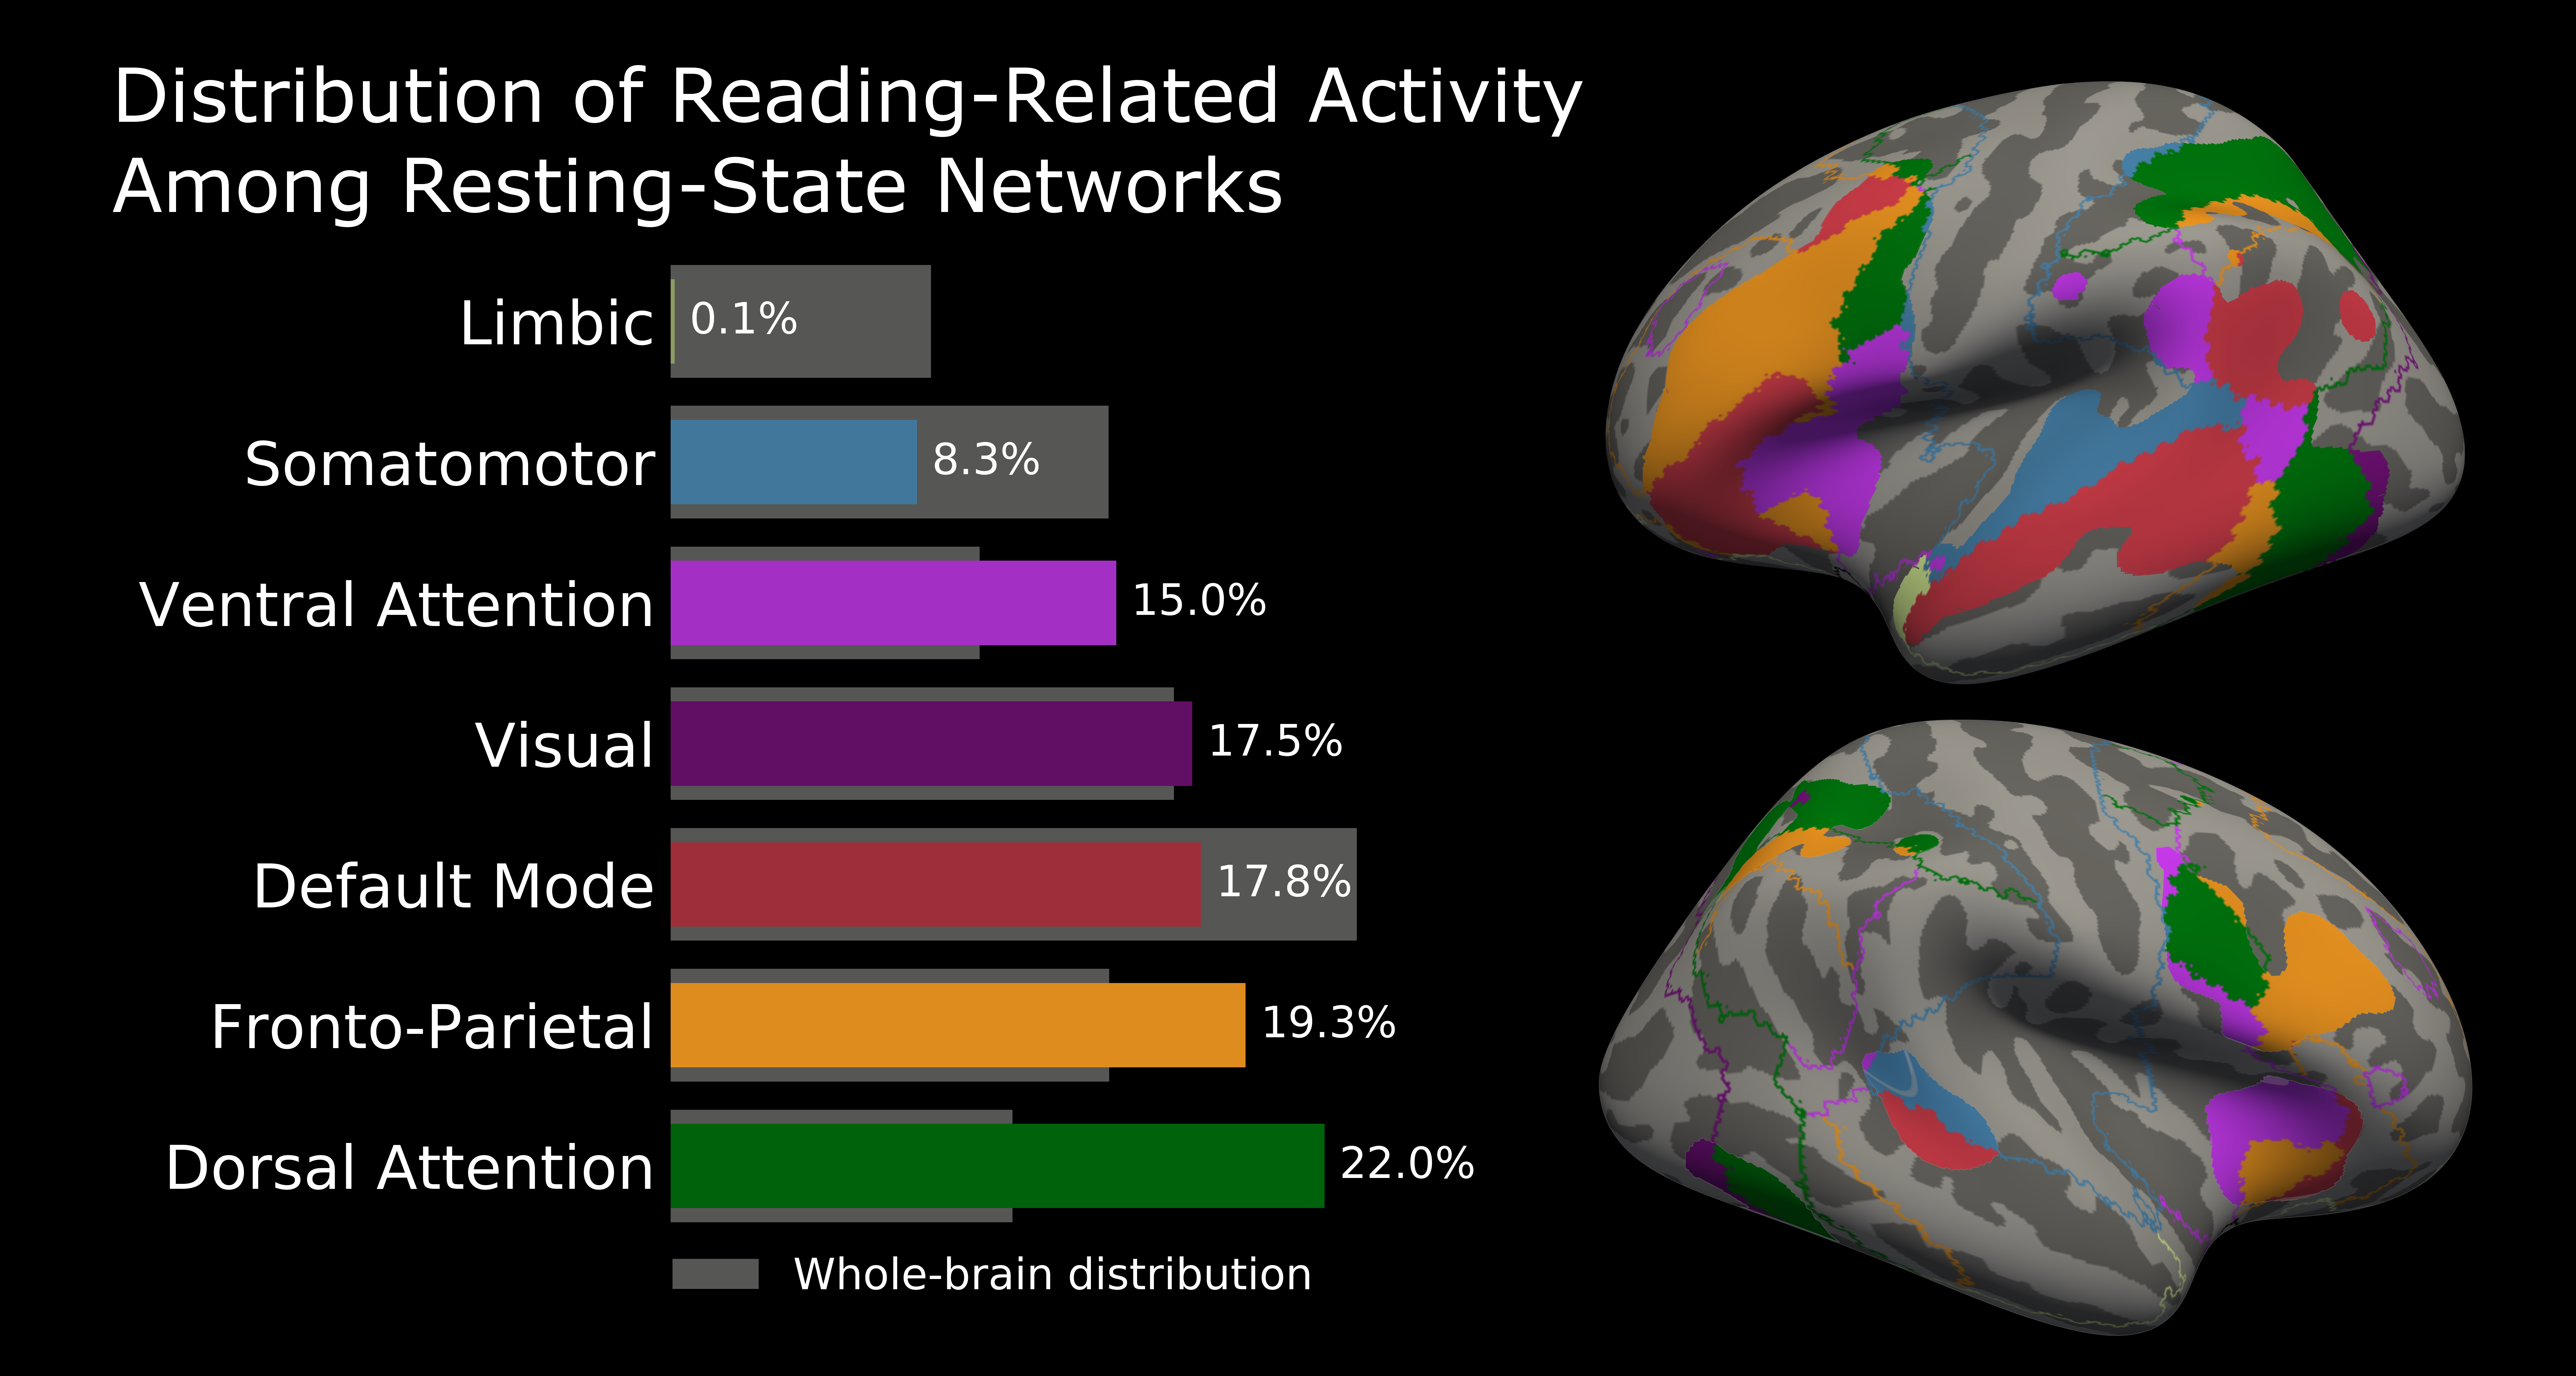
\includegraphics[height=3in]{images/ch1-yeo-to-neurosynth.png}
    \caption[Reading areas are distributed across many resting-state networks.]{Reading areas are distributed across many resting-state networks. On the left is the volumetric breakdown of the "reading" network, pulled from a NeuroSynth automated meta-analysis (forward-inference: $p < 0.01$, FDR-corrected) \citep{Yarkoni2011}, according to the 7-network cortical parcellation from Yeo and colleagues \citep{Yeo2011}. On the right is a surface plot of the same data. Reading areas are well-distributed across different networks and load highly onto attention and executive networks. Several important reading areas, including the inferior frontal gyrus and temporo-parietal junction, sit at points where multiple networks converge, i.e. likely hub areas.}
    \label{fig:ch1-yeo-to-neurosynth}
\end{figure}

\subsection{The visual word form area is part of the DAN} 
The visual word form area (VWFA) performs an important role in orthographic processing, and activity in the VWFA is sensitive to letter size, font and other orthographic attributes \citep{References from Vogel2011}. It's alleged specificity to language has been a source of controversy over the past decade \citep{...}, however, and several have argued that its importance in reading is directly linked to its membership in the DAN \citep{Vogel2014}. During reading, the DAN supports appropriate textual features or chunks and suppressing distracting information elsewhere \citep{Corbetta2002}. At issue in the debate is how general or specific visual attention deficits are in dyslexia \citep{Vogel2011}. Decreased activation in the pVWFA to text relative to typically developing participants has been reported in many studies of dyslexia \citep{...}, but these differences could be due to more generalizable visuo-spatial deficits. For example, fluent reading requires accurate and precise eye movements \citep{Rayner1998}, and a key node in the DAN is the "frontal eye fields" which help coordinate saccadic activity \citep{Petit1997,Connolly2000}. In fact, a number of studies report deficits in visual attention in children with RD (for a review, see Vidyasagar and Pammer 2010). Children with RD deficits in processing of consonant strings \citep{Pammer2004} and in matching symbol strings \citep{LassusSangosse2008}. Koyama et al. (2013) found that children with a historical diagnosis of dyslexia had persistant de-coupling of the dorsal attention network compared to typical readers regardless of remediation status \citep{Koyama2013}. Vogel et al. (2012) found that reading ability in typical children and adults (including decoding and passage comprehension ability) predicted increased correlations between the visual word form area and the dorsal attention network \citep{Vogel2012}. Whatever the true cause, it is clear that the DAN provides critical support for reading, above and beyond simply processing stimuli.

\subsection{Attention networks drive and suppress sensory integration} 
Attention underlies skilled reading at all levels: it is critical for identifying only the salient words in a large block of text, for suppressing environmental distractions and for maintaining focus for extended periods of time. In a common framework for attention, the dorsal and ventral attention networks (DAN and VAN) play collaborative roles for guiding focus. (The "salience" network, is sometimes differentiated from the VAN.) Simplistically, the DAN exerts top-down control of sensory processes to keep a person on task, while the VAN detects salient or unexpected stimuli, acting as a "circuit breaker" to help reorient the person \citep{Corbetta2002, Vossel2014}. This relationship may be impaired in individuals with dyslexia that have "sluggish attention shifting" attention between visual and auditory modality \citep{Harrar2014}. Slow or inadequately rapid attention-shifting could undermine fluent reading by causing temporal-spatial misalignment in processing, e.g. letter sequence and arrangement \citep{Lallier2009}. This deficit in attentional shifting is argued to further characterize dyslexic readers’ rapid temporal and low spatial frequency processing (e.g., \citep{Ingelhem2001, Witton1998}). Asynchronicity within this system is argued to be characteristic of dyslexia \citep{Vidyasagar2009, Lallier2009, Ingelhem2001}). Online interaction between the DAN and VAN during reading may thus index some of the attentional switching problems that are apparent in dyslexia. 

\subsection{Executive networks coordinate other cognitive processes} 
Executive functions play an important role in predicting reading outcomes, especially when considering comprehension \citep{Cutting2008}. Although the variety of cognitive processes that fall under EF construct do not map cleanly onto a single brain region or network, they are closely associated to the "central executive" system. This in turn is mapped on to the fronto-parietal network (FPN) (and sometimes the cingulo-opercular network) \citep{Fedorenko2013, Cocchi2013}. Unlike many other RSNs, the FPN has components which are not neighboring, spanning portions of the frontal and parietal lobes \citep{Yeo2011}. Interestingly, the FPN has recently been hypothesized to act as a neural mediator of other brain systems \citep{Mennon2010, Cole2014} by using wide-spread cortical connections to facilitate efficient processing of other networks, and in particular assist when areas are not functioning adequately. According to this coordinator model of the FPN, greater symptoms of dyslexia may correspond with reduced functional and structural integrity of the FPN. For instance, Norton et al. compared brain activation and connectivity in DYS reader sub-types, including readers with rapid naming deficits only, phonological awareness deficits only, and double deficits (i.e. poor rapid naming and phonological awareness) \citep{Norton2014}. They found graded de-activation and de-coupling of the FPN during a word rhyme judgment task, with the most severe deficit sub-group (double deficit) showing the greatest FPN de-activations and internal de-coupling. In the only functional connectomics paper on young readers with dyslexia, Finn et al. (2013) examined whole-brain connectivity during a word/non-word rhyming task, and found that children (and adults) with dyslexia showed de-coupling of frontoparietal areas \citep{Finn2013}. 

\subsection{Executive networks may support intervention response}
In addition to coordinating other RSNs, the FPN may play a role in supporting systems \citep{Cole2015}. Horowtiz-Kraus et al. (2015) examined resting state functional connectivity in young readers with and without dyslexia who had undergone a reading intervention \citep{HorowitzKraus2015}. They found that after intervention, readers with dyslexia had improved connectivity between a visual component and bilateral regions in the FPN (notably, as in many studies on reading, the latter component was not identified as an FPN component, but instead discussed as a language network). Furthermore, Koyama et al. (2013) examined resting state connectivity in dyslexic readers with variable remediation status, and found that children with a historical diagnosis of dyslexia had persistent de-coupling of frontoparietal areas compared to typical readers, regardless of remediation status \citep{Koyama2013}. Additionally, in the first reading study to examine functional interactions across networks, Aboud et al. (under review) found that, prior to intervention, readers who were responsive to the intervention mediated reading network connectivity via a key node in the FPN, the dorsolateral prefrontal cortex (dlPFC) \citep{Aboud2017_NF}. These findings support the hypothesis that executive areas in the FPN might act to facilitate the functional integrity of other systems necessary for reading.

\subsection{Default mode network engagement and disengagement} 
The DMN is a network of inter-connected regions (including medial prefrontal cortex, bilateral inferior parietal lobules, and posterior cingulate cortex) \citep{Shulman1997}. Since its original discovery, the DMN has since been found to support a wide range of cognitive processes often classified under internal mentation \citep{Buckner2008}, including theory of mind, narrative processing, and autobiographical recall \citep{AbdulSabur2014}. The DMN exhibits a large amount of overlap with traditional reading areas, including major comprehension-related regions such as the angular gyrus and anterior temporal pole. However, the DMN also has antagonistic relationship with "task-positive" attention networks such as the FPN, where the activation of one network necessarily comes at the suppression of the other, and this relationship appears to be important for performance on a variety of cognitive processes \citep{Fox2005, Keller2015}. Consequently, appropriate FPN involvement may be best achieved by suppression of the DMN. Several studies point to over-involvement of the DMN in readers with dyslexia, including higher internal correlations of the DMN during reading \citep{Finn2013} and greater correlations between the DMN and reading areas during reading and at rest \citep{Schurz2015}. Given that activity in both the FPN and DMN are critical for reading comprehension, understanding the dynamics of this relationship could be particularly illuminating.

\subsection{Hub areas show abnnormalities in dyslexia}
Two decades of neuroimaging research have allowed a relative consensus to form as to which brain regions are commonly dysfunctional in dyslexia. To determine whether there was any pattern related to network architecture in these areas, we gathered all clusters from three meta-analyses comparing fMRI activation for individuals with dyslexia to typical readers \citep{Maisog2008, Richlan2009, Paulesu2014}. All areas that showed atypical activation in dyslexia (either greater or less activity) were included. When a cluster was large, all reported local maxima were included. 

To get measures of hubness across the brain, we used data from a connectomics study by Power and colleagues (2013) \citep{Power2013}. That study reports the \textit{participation coefficient} for each of the 264 nodes previously described. The participation coefficient reflects the diversity of a node's connectivity to different RSNs, where a higher value indicates that the node is correlated with many different RSNs. Activations from the dyslexia meta-analyses were then mapped to the geometrically closest node from this dataset, resulting in a small set of dyslexia-related nodes and a larger, unaffected set.

The distribution of participation coefficients across the 264 nodes was non-normal, with a large group of areas having low participation coefficients (i.e. affiliated with few RSNs) and a smaller hub-like group. Therefore, a Wilcoxon rank-sum test was performed on the participation coefficients for the two groups, which tests for the equivalence of two distributions in a non-parametric fashion.

Across the three meta-analyses, 32 of the 264 nodes showed abnormal functioning in dyslexia. Figure 3 shows the node-by-node distribution of participation coefficients for the entire set. The median participation coefficient for unaffected nodes was 1.47; for dyslexia-related nodes it was 3.28. A Wilcoxon rank-sum test between the dyslexia and unaffected nodes showed that dyslexia affects brain areas with higher participation coefficients than would otherwise be expected ($U = 4946.0$, $p$ \textless $0.001$). 

\begin{figure}[h!]
\centering
\includegraphics[height=3in]{images/ch1-dyslexia-hubs.png}
    \caption[Dyslexia disproportionately impacts hub areas.]{Dyslexia disproportionately impacts hub areas. Among the brain areas examined in Power and colleagues (2013), nodes implicated in dyslexia have higher participation coefficients (32 nodes) compared to the rest of the brain (232 nodes).}
\label{fig:ch1-dyslexia-hubs}
\end{figure}

\section{Influence of development on network connectivity}

Children are taught to decode words between the ages of four and nine. This is a time of major developmental changes in the brain, with extensive synaptic pruning and myelination of white matter tracts \citep{Wandell2013}. The brain areas responsible for fast and efficient word decoding may become specialized through a process of \textit{interactive specialization}, in which intrinsic developmental processes and experience collaborate to form the mature, skilled reading system \citep{Johnson2011, Klingberg2014}. The theory is an extension of the Hebbian maxim that "neurons that fire together, wire together", with the brain being considerably more plastic during this developmental period than it is later in life \citep{Hebb1949}.

\begin{figure}[h!]
\centering
\includegraphics[height=3in]{images/ch1-interactive-specialization.jpg}
    \caption[Interactive specialization explains changes in activity.]{Interactive specialization posits that repeated co-activation of distant brain areas will create a network of regions important for performance of a given task. Figure taken from \citep{Gaffrey2012}.}
\label{fig:ch1-interactive-specialization}
\end{figure}

This process of interactive specialization may cause lasting changes to connectivity even when subjects are not reading. Evidence for this comes from resting-state fMRI, which does not require individuals to complete tasks but instead uses spontaneous neural activity from the fMRI signal to construct networks. Koyama et al. found that many reading-related nodes had overlapping connectivity with the left inferior frontal gyrus and left middle temporal gyrus, both nodes that are important for skilled language use \citep{Koyama2010}. A follow-up study comparing IQ-matched children and adults found similar patterns: better readers in both groups showed increased connectivity between the inferior frontal gyrus and the middle and superior temporal gyri, as well as between the precentral gyrus and motor areas \citep{Koyama2011}. In adults, positive correlations were found between reading ability and connectivity between the visual word form area and phonological processing areas; in children, however, this correlation was weaker and negative, suggesting that the visual word form area becomes more integrated with experience as well as skill. Reading intervention also exerts an effect on connectivity patterns. Dyslexic adolescents who received reading remediation had higher correlations between the visual word form area and the right middle occipital gyrus than did control participants \citep{Koyama2013}. This connectivity also correlated with spelling and single-word reading scores.

However, word recognition skill is insufficient to explain individual differences in comprehension \citep{Gough1986, Hoover1990}. That is, comprehension requires more areas of the brain than do those of more basic reading skills. Multiple studies have shown that in single-word reading tasks, neural activity is largely confined to areas near the visual system in fusiform regions, whereas in sentence and passage comprehension, readers utilize a broader array of brain regions \citep{Rimrodt2008,Xu2005}. Other reports corroborate these larger activations: Cutting et al. used a sentence comprehension task which elicited bilateral temporal lobe activation (left \textgreater right) and greater occipital lobe signal, as would be expected from increased language and visual load. Thus, sentence comprehension relies on a core set of extended language regions above that required for words.  \citep{Cutting2006a}. Consistent with theory, as readers become more skilled, patterns become more focused and sharply defined; in contrast, those who continue to struggle with reading (i.e. dyslexia) continue to show a more diffuse pattern of activity \citep{Rimrodt2009}. 

Relatively few studies have been done relating network methods to reading ability. Despite the changes in connectivity between areas, reading-related regions such as the fusiform gyrus, angular gyrus and inferior frontal gyrus, do not create one distinct RSN, but are members of separate, more primary RSNs \citep{Vogel2013}. Finn et al. compared graph theory metrics of dyslexic and non-impaired readers using graph metrics \citep{Finn2014}. Dyslexic readers showed divergent activity in visual association and prefrontal attention areas as well as increased right-hemisphere connectivity. Differences were persistent across both adult and children readers, suggesting that network metrics are relevant for reading. Another study investigating how graph theory metrics changed in response to sentence-level processing showed that network properties were relatively stable \citep{Ye2012}. Participants were asked to silently read a sentence that had either a semantically congruent or incongruent ending. Furthermore, metrics showed that subcortical processing (basal ganglia to supplementary motor area) was stronger in response to incongruent versus congruent endings. 

According to the view of interactive specialization, an integrative ability like reading comprehension would be more highly connected. The multi-RSN robustness, or the how well-maintained the network is after deletion of a node, will measure how strongly inter-connected the RSNs of interest are to each other \citep{Bullmore2009}. An important consequence of these hypotheses is that, if there is a biological substrate underlying RC, we may have another window into predicting how well a child will continue to develop as a reader, especially during the periods of rapid development in primary school.


\section{Conclusions}


We have establisehd that the network model for reading has particular bearing in models of reading, and that graph theory methods provide a summary framework with which to investigate the interactions between processes. Furthermore, development of cognitive skills is facilitated by the interactions between regions, rather than solely by themselves - but the study of these processes have not been investigated extensively. 

In this dissertation, I present three studies that investigate network properties as they relate to reading comprehension and reading success. The common thread is that reading requires the integration of many different brain networks (even moreso than listening) and that better readers are more able to meet these demands, even from a young age.

\begin{itemize}
    \item \textit{Study 1} investigates differences in global network topology between reading and listening and then hones in on changes to executive and attention networks 
    \item \textit{Study 2} looks at changes to whole-brain connectivity patterns in reading comprehension throughout development using a cohort of subjects aged 8 to 28
    \item \textit{Study 3} investigates individual differences in reading skill and its relationship to "intrinsic" network topology, using a large resting-state fMRI dataset with subjects spanning the many stages of development
\end{itemize}

Throughout, I will be leveraging fMRI and behavioral data collected in the Education and Brain Sciences Research Laboratory at Vanderbilt University. 


\chapter{Reorganization of network architecture during reading and listening}

\epigraph{Reading is parasitic on language... [It] is seen not as a parallel activity in the visual mode to speech perception in the auditory mode: there are differences... [that] can be explained only if we regard reading as a deliberately acquired, language-based skill, dependent up on the speaker-hearer's awareness of certain aspects of primary linguistic activity.}{I. Mattingly, 1972 \citep{Mattingly1972}}

\section{Motivation}

In the first chapter, we established that reading utilizes a variety of cognitive skills whose neural substrates are distributed throughout the brain. But being able to comprehend speech is a pre-requisite to reading, and it is similarly complex. This begs the question: in what ways is reading unique from listening?

The most widely-held view is that reading and listening share the same core linguistic processes and differ primarily in the sensory processes that feed into supra-model linguistic systems \citep{Mattingly1972, Price2012}. One popular model, the \textit{Simple View of Reading} states that reading comprehension is the product of listening comprehension and decoding skills \citep{Gough1988}. This view has received support from large behavioral studies \citep{Kirby2006} and neuroimaging investigations: many of the literacy-related changesare linked to visual or phonological systems, areas not directly related to semantic or comprehension processes \citep{Schlaggar2006, Dahaene2015}. These findings support a model in which inputs from auditory or visual domains are fed up into higher-order association areas that sequence, encode articulatory plans, and extract semantic information \citep{Price2012}. These processes localize onto the similar areas regardless of language and writing system \citep{Rueckl2016}, and may even extend to inputs from somatosensory domains \citep{Xu2005, Sood2015}. This supra-modal language core is largely left-lateralized and centers on the inferior frontal gyrus, anterior and posterior middle temporal gyrus and the angular gyrus. Neuroanatomical models of language, shown in Fig. \ref{ch2-price-language-models}, illustrate that language is distributed throughout much of the brain. 

\begin{figure}[t]
	\centering
	\includegraphics[height=3in]{images/ch2-price-language-models.jpg}
	\caption[Schematics of skills and brain areas used in reading.]{Models of reading typically focus on a common linguistic core that is responsible for comprehension and production of language. In this model, differences in modality affect input pathways to this core.}
	\label{fig:ch2-price-language-models}
\end{figure}

Despite the clear overlap between reading and listening, there is also evidence that the two skills are not directly equivalent. There is a subset of students who, despite adequate word decoding skills and vocabulary skills, struggle with reading comprehension\citep{Nation2010, Spencer2011}. From a neurobiological perspective, expected differences in primary visual (for reading) and primary auditory (for listening) represent the different input systems, with ventral occipito-temporal systems also activating \citep{Jobard2007}. However, differences in core language systems are also observed: additional activation in left posterior temporal and parietal areas in reading modality \citep{Constable2015}, as well increased bi-laterality especially in children \citep{Berl2010}. 

Most current cognitive models suggest that language comprehension requires the construction of a mental representation includes textual information and associated background knowledge, connected by some conscious and some unconscious executive processes \citep{Kendou2014}. The parallel model shown in Fig. \ref{fig:ch2-price-language-models} is linear: it moves from sensation to action. During comprehension, however, the relationship between areas is dynamic and constantly being re-evaluated. The roles of attention and executive systems are likely to play an important role. Thus, while there may be a core set of systems for manipulating and extracting meaning from language, it is likely that differences in modality would modulate these processes. 

The pioneering researcher Alvin Liberman suggested that reading, instead of being parallel to listening, is actually parasitic: it requires an textit{awareness} of the linguistic act that is not required in listening. Brain activation studies may not capture these differences: it could very well be the interactions of different functional systems that are changed, rather than the overall "engagement" of an individual brain area. Additionally, the fact that reading integrates in an additinoal modality could be a source of difference, especially in emerging readers. 

% \subsection{How the brain reconfigures (Cohen + Esposito)}
% A critical feature of the human brain that gives rise to complex cognition is its ability to reconfigure its network structure dynamically and adaptively in response to the environment. Existing research probing task-related reconfiguration of brain network structure has con-cluded that, although there are many similarities in network structure during an intrinsic, resting state and during the performance of a variety of cognitive tasks, there are meaningful differences as well. In this study, we related intrinsic, resting state network organization to reconfigured network organization during the performance of two tasks: a sequence tapping task, which is thought to probe motor execution and likely engages a single brain network, and an n-back task, which is thought to probe working memory and likely requires coordination across multiple networks. We implemented graph theoretical analyses using functional connectivity data from fMRI scans to calculate whole-brain measures of network organization in healthy young adults. We focused on quantifying measures of network segregation (modularity, system segregation, local efficiency, number of provincial hub nodes) and measures of network integration (global efficiency, number of connector hub nodes). Using these measures, we found converging evidence that local, within-network communication is critical for motor execution, whereas integrative, between-network communication is critical for working memory. These results confirm that the human brain has the remarkable ability to reconfigure its large-scale organization dynamically in response to current cognitive demands and that interpreting reconfiguration in terms of network segregation and integration may shed light on the optimal network structures underlying successful cognition.
%
% We know that the single most important function in reading is \textit{decoding} visual stimuli into linguistic representations of words. Mastering this process creates permanent changes to brain structure and function, as well as to behavioral responses to speech. The dominant ``parallel'' model of reading suggests that this symbol-to-speech mapping process is the principal difference between reading and listening; that after feeding input ''up'' from visual or auditory systems, the linguistic processes are the same. However, many children struggle to comprehend text even after becoming proficient decoders, and there are clear differences in the nature of the modalities, including grammar, motor processes (e.g. eye movements), and differences in contextual information available (e.g. pitch, tone, rhythm in listening; peripheral words, recursive glances in reading). Therefore, decoding is not the only process that makes reading different from listening, but it is not clear which other cognitive processes might most contribute to reading success or failure. ...The ``parasitic'' model of reading asserts that reading is a skill built on top of the linguistic process \citep{Mattingly1972}. 



In this study, we pursue three hypothesized ways reading might differ from listening. These are not exclusive; one or more of them may be true. The overarching aim is to test whether reading and listening differ only, or primarily, in their 

\begin{itemize}
	\item Reading will require a greater "global" reorganization of resting-state networks than listening. This network will also be more highly integrated than that of listening. 
	\item Reading will reduce the modularity within the sensory system of interest. That is, visual areas will become less internally connected during reading, while auditory areas will be less internally connected during listening.
	\item Reading will make greater demands on attention systems than listening. That is, areas in the frontal and attention systems will be activated to a greater degree during reading than listening.
\end{itemize}

First, we validate modularity and participation coefficient metrics using univariate data, and test that language induces greater global integration, especially in higher-order networks (executive and attention) compared to resting and attention baselines. Second, we test three hypotheses about how interactions between brain networks might differ from speech.


\section{Methods}

The following methods detail the current study's protocol and analytical approach. The following chapters borrow heavily from the methods described below, so they are explained here in detail. 

\subsection{Participants}

Participants for the first study were drawn from the fourth wave of a larger, longitudinal study investigating the neurobiological bases of reading comprehension. 52 children completed scans for the current study and a subset of these met the motion and attention thresholds described below. See Table \ref{table:ch2-participants} for demographics. 

All participants were native English speakers with normal hearing and normal or corrected vision, and no history of major psychiatric illness or traumatic brain injury/epilepsy. Subjects had no history of a developmental disability or contra-indication to MRI.  Each participant gave written consent at the beginning of the study, with procedures carried out in accordance with Vanderbilt University’s Institutional Review Board.

\begin{table}
	\renewcommand{\tabcolsep}{0.09cm}
	\centering
	\begin{tabular}{lc}
\toprule 
Measure & Subjects \\ 
\midrule 
No. Participants				& 42 \\ 
No. Scan Runs					& 164 \\ 
Gender  						& 25 F \\ 
Age at Scan 					& 10.5 (0.3)  \\ 
WASI Full-Scale IQ  			& 111.0 (16.2) \\ 
TOWRE - Total Word Efficiency 	& 104.6 (18.5) \\ 
\bottomrule 
\end{tabular}
	\caption[Participant demographics for Study 1.]{}
	\label{table:ch2-participants}
\end{table}

\subsection{Functional MRI Task}

We designed an fMRI task in which participants either read or listened to a passage of text. The passage was split into two paragraphs and interspersed with a simple attention task. At the end of the task, there was an approximately three minute long resting-state block. Across runs, conditions were presented in the same order, although durations varied slightly. Condition order was: comprehension block (paragraph 1), sensory baseline (set 1), comprehension block (paragraph 2), sensory baseline, and resting baseline. See Fig. \ref{fig:ch2-task-design} for a schematic.

\begin{figure}[t]
	\centering
	\includegraphics[height=3in]{images/ch2-eprime-recall.png}
	\caption[Schematic of the reading comprehension task.]{}
	\label{fig:ch2-task-design}
\end{figure}

To create a more naturalistic reading experience than single word presentation \citep{Rayner1986}, passages were presented in syntactic phrases ranging from 1-7 words in length. The interval between each stimulus was jittered to allow for event-related analyses (range: 275 – 4000 ms), although these effects were not examined here.

The sensory baseline condition was altered according to modality. For the reading runs, three non-alphanumeric symbols were displayed horizontally (two types), and their presentation time was matched to the passage phrases. Spacing between symbols was randomly alternated to replicate the variable phrase lengths in the passage condition. For the listening runs, three tones (two frequencies) were played in sequence, with a new set of tones beginning at the same intervals as the corresponding passage presentation. 

To monitor attention, 4 to 8 percent of the stimuli within each passage or attention block were randomly repeated on two consecutive screens.  Participants pressed a button with their right thumb when they detected a repeated phrase, symbol or tone configuration. Additionally, at the conclusion of each passage, a picture was presented on the screen, and subjects were asked to identify whether the picture had any relationship to the passage (e.g., a picture of a mushroom for a passage about fungi). 

To assess performance, we analyzed three measures: in-scanner attention, in-scanner comprehension, and post-scan recall. To assess attention, we calculated the $D`$ statistic ($Z(true\ positive) - Z(false\ positive)$) for the "repeated stimulus" task. The in-scanner comprehension measure was the number (0,1,2) of questions correclty answered. To assess recall, each child was asked to recite as much of the passage as they could remember, and their answers were mapped to actual phrases present in the chapter. Individual scan runs with a $D`$ value less than 2 were excluded from analysis.

In total, there were 4 passages (2 listening, 2 reading), each leveled to a 3\textsuperscript{rd} grade difficulty and balanced on word measures such as concreteness and cohesiveness.  All subjects were trained on the task in a mock scanner prior to the actual scan. 


\subsection{MRI acquisition}

Imaging was performed on a Philips Achieva 3T MR scanner with a 32-channel head coil. Functional images were acquired using a gradient echo planar imaging sequence with 40 (3 mm thick) slices with no gap. Each run of the task (up to four) consisted of 250 volumes. Slices were parallel to the anterior-posterior commissure plane. Imaging parameters for functional images included: TE = 30 ms; FOV = 240 x 240 x 120 mm\textsuperscript{3}; flip angle = 75\degree; TR = 2200 ms; and 3 mm\textsuperscript{3} isotropic voxels.

\subsection{Activation analyses}

Whole-brain fMRI analyses were performed using tools from the FMRIB Software Library (version 5.0.9). For each session, the following pre-processing steps were performed:  slice-time correction, motion correction to the initial fMRI volume, high-pass filtering at 0.08 Hz, boundary-based registration to the subject's structural image, and normalization to 2 mm MNI 152 standard space. To mitigate the effects of motion on our analyses, we regressed out 6 continuous motion parameters and scrubbed out outlier volumes. We defined an outlier volume as any in which the root-mean-square framewise displacement exceeded 0.7 mm. Because head motion can be a major confound for connectivity analyses, we removed scan runs where more than 10 percent of the fMRI volumes were outliers.

All task conditions were convolved with the double-gamma hemodynamic response function to generate design matrices for each fMRI run. Two first-level contrasts were of interest: the main effect of passage comprehension (“pass vs. rest), and the contrast of passage comprehension vs. the sensory baseline ("pass vs. attn."). Repeated stimuli and the picture comprehension task were modelled out.

Modality effects (Shared Effect of Listening and Reading, Contrast of Listening and Reading) were estimated at the subject-level using fixed effects analysis. These were carried over into group-level analyses using non-parametric methods implemented in FSL’s \textit{randomise} tool with threshold-free cluster enhancement. For each group-level analysis, we performed 10,000 permutations and report results with \textit{p} \textless 0.05. 

\subsection{Connectome analyses}

To investigate whole-brain patterns of connectivity without biasing our results towards our task, we selected 264 nodes \textit{a priori} whose connectivity properties have been extensively analyzed \citep{Power2011}. This node set samples the entire brain and are involved in a diversity of cognitive tasks. Each node was assigned to one of 13 RSNs based on previous literature \citep{Power2013}. Approximately 10 percent of the nodes did not have a stable assignment in the original paper; for the present analyses, these nodes were excluded from graph theory calculations. A description of the 13 networks, their size, and their overlap with the 2011 Yeo parcellation is provided in \ref{table:ch2-power-nodes}. 

\begin{table}
	\renewcommand{\tabcolsep}{0.09cm}
	\centering
	\begin{tabular}{lcc}
\toprule 
Suggested RSN & Abbreviation & Nodes \\ 
\midrule 
\textit{Sensory} & & \\
	\hspace{3pt}Auditory  			&  AUD & 13 \\ 
	\hspace{3pt}Somatomotor (Hand)	&  SOH & 30 \\
	\hspace{3pt}Somatomotor (Mouth)	&  SOM & 5 \\
	\hspace{3pt}Visual	 			&  VIS & 31 \\ 
\textit{Attention} & & \\
	\hspace{3pt}Dorsal attention  	&  DAN & 11	\\ 
	\hspace{3pt}Salience		  	&  SAL & 18 \\ 
	\hspace{3pt}Ventral attention  	&  VAN & 9 \\ 
\textit{Executive} & & \\
	\hspace{3pt}Cingulo-opercular 	& CON & 14 \\ 
	\hspace{3pt}Default mode		& DMN & 58 \\
	\hspace{3pt}Fronto-parietal  	& FPN & 25 \\ 
	\hspace{3pt}Memory retrieval	& MEM & 5 \\
\textit{Other} & & \\
	\hspace{3pt}Cerebellar			& CER & 4  \\
	\hspace{3pt}Subcortical			& SUB & 13 \\
	\hspace{3pt}Not assigned 		& UNC & 28 \\ 
\bottomrule 
\end{tabular}
	\caption{Networks used in connectivity analyses.}
	\label{table:ch2-power-nodes}
\end{table}

To understand our univariate results as a function of RSN activation, we cast the activations into connectome space and reviewed each contrast according to the network affiliation of the corresponding nodes.

For graph theory analyses, network estimation was performed in the \textit{Conn: Functional Connectivity Toolbox} (version 17f) \citep{Nieto-castanon}. For each scan run, the BOLD activity at each node was denoised using the anatomical CompCorr method, which regresses out background noise from white matter and cerebrospinal fluid tissue. We also regressed out 12 continuous measures of motion were also included, all outlier timepoints, and the effect of all task conditions ("pass", "attn", "rest"). The timeseries was then high-pass filtered at 0.01 Hz.

Whole-brain connectomes for each condition were created by estimating the functional connectivity between each node using a weighted general linear model. For connection-level analyses, these values were compared directly across subjects and conditions. For graph theory analyses, the array of all node connections was thresholded to keep the top 5 percent of connections, resulting in a much sparser representation. This threshold was also tested at ranges from 2 percent to 10 percent, and all reported results were significant at the reported level in at least 7 of the 9 tested thresholds.

The metrics of interest were network \textit{modularity}, \textit{participation coefficient} and \textit{path length}. Modularity is high in networks where nodes within the same RSN are highly connected to each other but not elsewhere. The participation coefficient, on the other hand, is high when many nodes are connected to several different RSNs. Both of these metrics relate to the integration of information between RSNs. Path length, on the other hand, describes the distance between any two nodes on the graph. This was calculated between every node, then summed up by RSN to create a measure of network distance. These properties, and their changes within our task, were investigated at the level of connectomes, RSNs and nodes. 


\section{Results}

\subsection{Behavioral results}

42 subjects (142 scan runs) met the attention and motion criteria to be included in the analysis. (10 subjects and 61 individual scan runs were filtered out.) Attention and comprehension measures were not related to modality of stimulus presentation (see Fig. \ref{fig:ch2-task-performance}). There was a trend towards difference in median FDRMS between scan modalities (paired t-test, $t = 1.94$, $p = 0.059$), so we also replicated analyses with a stricter motion threshold (no more than 10 percent outliers in a scan run). The main results from analysis of this 35 subject (116 scan runs) cohort were broadly consistent.

\begin{figure}[t]
	\centering
	\includegraphics[height=3in]{ch2-task-performance}
    \caption[Behavioral metrics of passage performance were unrelated to modality.]{Both the in-scanner comprehension question and out-of-scanner recall questionnaire were unrelated to the modality of presentation.}
	\label{fig:ch2-task-performance}
\end{figure}

\subsection{Activation results}

A range of language-related areas were activated for both reading and listening comprehension (Fig. \ref{fig:ch2-passages-activation-attn}). Compared to the corresponding sensory baselines, activation spanned the inferior frontal gyrus, angular gyrus, premotor cortex, middle temporal gyrus and the superior frontal gyrus. Activation patterns were robustly present on both hemispheres, but had greater intensity and extent on the left hemisphere. 

\begin{figure}[t]
	\centering
	\includegraphics[height=3in]{ch2-passages-activation-attn}
    \caption[There is significant overlap between the areas used in listening and reading.]{A widespread set of brain areas are utilized during listening and reading, including auditory, default mode and attention areas.}
	\label{fig:ch2-passages-activation-attn}
\end{figure}

Differences related to modality fell into three categories: sensory processing areas, including the insula, superior temporal gyrus, and secondary visual processing areas; and hetero-modal association areas, most notably the inferior frontal gyrus and angular gyrus; and somato-motor regions, including the premotor cortex and lateral geniculate nucleus of the thalamus (Fig. \ref{fig:ch2-modality-differences-attn}). Areas showing greater activation in listening were focused on primary auditory cortex and the dorsal attention network.

\begin{figure}[t]
	\centering
	\includegraphics[height=3in]{ch2-modality-differences-attn}
    \caption[Modality differences center on primary sensory and integration areas.]{Visual and sensory association areas were higher in reading, while listening showed increased activity in auditory and dorsal attention network areas.}
	\label{fig:ch2-modality-differences-attn}
\end{figure}

We also examined these contrast results when projected onto the 264-node connectome. There was a high degree of similarity between the areas that were activated in reading and in listening, reflecting the common language core. Fig. \ref{fig:ch2-listening-reading-connectome-activations} shows the activation statistics for each node, relative to rest, plotted against each other. There was a very high correlation coefficient ($r = 0.00$), reflecting the high degree of shared activity patterns between listening and reading.

\begin{figure}[t]
	\centering
	\includegraphics[height=3in]{ch2-listening-reading-connectome-activations}
    \caption[There is significant overlap between the areas used in listening and reading.]{A widespread set of brain areas are utilized during listening and reading, including auditory, default mode and attention areas.}
	\label{fig:ch2-listening-reading-connectome-activations}
\end{figure}

Comparing the modality difference statistics within each network revealed that the visual RSN is much more active during reading than listening, but that some, but that the dorsal attention network was more active during listening.

\begin{figure}[t]
	\centering
	\includegraphics[height=3in]{ch2-modality-stripplot-connectome}
	\caption[Modality differences show RSN-level trends.]{}
	\label{fig:ch2-modality-stripplot-connectome}
\end{figure}[t]


\subsection{Graph theory results}

Next, we examined changes to the global graph theory measures. Figure \ref{fig:ch2-comprehension-graph-theory} displays the changes in modularity and participation coefficient at the subject-level. Relative to rest, both listening and reading reduced the global modularity and increased the participation coefficient. Compared to the baseline attention task, there was  a trend towards an increased participation coefficient, but it was not significant. 

\begin{figure}[t]
	\centering
	\includegraphics[height=3in]{ch2-comprehension-graph-theory}
    \caption[Language induces more integrated global network architecture.]{Compared to rest and baseline attention tasks, reading and listening increase measures related to global RSN integration.}
	\label{fig:ch2-comprehension-graph-theory}
\end{figure}

A direct comparison of listening to reading showed that reading induced a more integrated network architecture than listening, both in terms of reduced modularity and increased participation coefficient (Fig. \ref{fig:ch2-modality-graph-theory}).

\begin{figure}[t]
	\centering
	\includegraphics[height=3in]{ch2-modality-graph-theory}
    \caption[Reading is more integrated than listening.]{}
	\label{fig:ch2-modality-graph-theory}
\end{figure}

Investigating these graph theory measures at the level of RSN provides  insight as to which networks are driving the changes in integration. When comparing comprehension differences to rest, for example, we can see that globally connectivity increases (Fig. \ref{fig:ch2-comprehension-reorganization}. During rest, however, there is increased connectivity within default mode network and visual networks.

As would be expected, the visual network undergoes large changes in reading: specifically, there is a large decrease in visual-visual connectivity. 

To investigate interactions between networks, rather than simply general behavior of the networks, we summarized the average shortest path length between each network. This provides a gross measure of how close any two networks are. 

In the case of comprehension, we found that there was lower path length within modules during rest, while there were decreases in between-network connectivity during language.

For the modality contrast, One of the main takeaways is that there is greater access between auditory and other areas during reading -- this runs counter to our hypothesis that there would be less access to these areas. Visual areas, on the other hand, show less internal connectivity, reflecting the de-clustering of these areas during reading. 

\begin{figure}[t]
	\centering
	\includegraphics[height=3in]{ch2-modality-node-distance}
    \caption[Summary of the change in distance between nodes during reading and listening.]{}
	\label{fig:ch2-comprehension-reorganization}
\end{figure}

\begin{figure}[t]
	\centering
	\includegraphics[height=3in]{ch2-comprehension-reorganization}
    \caption[Language increases between-network connectivity.]{}
	\label{fig:ch2-comprehension-reorganization}
\end{figure}


\begin{figure}[t]
	\centering
	\includegraphics[height=3in]{ch2-modality-reorganization}
    \caption[Reading decreases connectivity within visual and dorsal attention networks.]{}
	\label{fig:ch2-modality-reorganization}
\end{figure}


\section{Discussion}

This study investigates the differences between reading and listening in terms of their activation of individual areas or the distribution of activity across the brain. We employ closely matched texts, large sample size, longitudinal sampling, and behavioral covariates. Comprehending extended text requires more than just sensory and linguistic processes. It also requires executive processes such as attention, working memory and inference. Since comprehension is a "whole-brain" activity, we here look at the reorganization of resting-state networks - to see how attention, executive and sensory systems are interacting during reading.

The results make clear that differences in reading are not isolated solely to sensory systems, although the visual system is the major driver. We tested three hypotheses related to global reorganization, sensory system changes, and interactions between executive and attention systems and sensory systems.

These modality-specific influences on behavior and brain activity may arise from a few different sources: subject, linguistic and innate differences. For example, there are also differences in what is encoded in speech and text. The reading sciences pioneer Alvin Liberman noted that "speech is a complex code, while reading is a simple cipher" \cite{Mattingly1972}. Speech contains overt clues about the speaker, such as tone and prosody, and these can convey additional non-linguistic meaning for the listener. Reading, on the other hand, might be considered a more purely linguistic act, especially with computer-printed text. Reading may thus allow more room for self-generated situation models and more independent direction of thought. Furthermore, modality-specific aspects of the stimulus may influence the overall comprehension process; reading requires a level of spatial awareness -where one is at on a page, what happened in preceding paragraphs – and allows for the re-treading of information. Listening, meanwhile, requires the extraction of input from competing noises and sometimes the tracking of changing volume. 

People speak differently than they write. Reading often relies on more complicated syntax, and even for skilled readers, longer words and sentences can strain executive systems more than they might if being spoken to. Although these properties are often controlled for in scientific studies, they represent a major difference between “natural” reading and listening. Because of these differences, reading may place a greater load on executive function skills. Executive functions such as working memory and planning and organizing may be particularly important for reading \citep{Cain}.  

\begin{table}
	\renewcommand{\tabcolsep}{0.09cm}
	\centering
	\begin{tabular}{ll}
\toprule 
Finding & Figure(s) \\ 
\midrule 
Reading and listening share supra-modal lingage core.	& \ref{fig:ch2-passages-activation-attn} \\ 
Reading shows greater activation in many linguistic areas.	& \ref{} \\ 
Language increases connectivity between RSNs globally, compared to rest and baseline attention.	& \ref{} \\ 
Reading has higher integration, drivn largely by de-clustering of visual areas.	& \ref{}  \\ 
Decreased distance between sensory and attention areas.  &  \ref{} \\ 
\bottomrule 
\end{tabular}
	\caption[Summary of findings for Study 1.]{}
	\label{table:ch2-results}
\end{table}

The last set of differences is particularly interesting because knowing how the differences in reading interact with these modality differences. Reading is a learned skill with may component processes. It requires thousands of hours of experience to master and entails a reorganization of cortical resources. Environmental and biological factors thus exert a greater influence on an individual’s reading proficiency than they might on more intrinsic processes such as speech comprehension. This is particularly dramatic in individuals with dyslexia, who have persistent difficulty with reading. Children with dyslexia exhibit less activation in reading-related areas compared to typically developing children \citep{Pugh2000}, but greater activation in right hemisphere homologues, suggesting that lateralization and activation of the reading circuit are associated with better reading. Development period also has an effect, with children exhibiting less activation in frontal areas but more in posterior areas, possibly reflecting a shift in “resource load” from uni-modal to supramodal areas \citep{Berl2010}. This shift may not be necessary in listening, or occur much earlier. Thus, with increasing expertise and development, there may be a “shift” from relying on fusiform processing areas. towards using multi-modal areas more like speech \citep{Monzalvo}. 

This interaction between reading activation and individual differences in maturity and reading skill will be the subject of the next chapter.
\chapter{Reorganization of network architecture during reading and listening}

\epigraph{Reading is parasitic on language... [It] is seen not as a parallel activity in the visual mode to speech perception in the auditory mode: there are differences... [that] can be explained only if we regard reading as a deliberately acquired, language-based skill, dependent up on the speaker-hearer's awareness of certain aspects of primary linguistic activity.}{I. Mattingly, 1972 \citep{Mattingly1972}}

\section{Motivation}

In the first chapter, we established that reading utilizes a variety of cognitive skills whose neural substrates are distributed throughout the brain. But being able to comprehend speech is a pre-requisite to reading, and it is similarly complex. This begs the question: in what ways is reading unique from listening?

The most widely-held view is that reading and listening share the same core linguistic processes and differ primarily in the sensory processes that feed into supra-model linguistic systems \citep{Mattingly1972, Price2012}. One popular model, the \textit{Simple View of Reading} states that reading comprehension is the product of listening comprehension and decoding skills \citep{Gough1988}. This view has received support from large behavioral studies \citep{Kirby2006} and neuroimaging investigations: many of the literacy-related changesare linked to visual or phonological systems, areas not directly related to semantic or comprehension processes \citep{Schlaggar2006, Dahaene2015}. These findings support a model in which inputs from auditory or visual domains are fed up into higher-order association areas that sequence, encode articulatory plans, and extract semantic information \citep{Price2012}. These processes localize onto the similar areas regardless of language and writing system \citep{Rueckl2016}, and may even extend to inputs from somatosensory domains \citep{Xu2005, Sood2015}. This supra-modal language core is largely left-lateralized and centers on the inferior frontal gyrus, anterior and posterior middle temporal gyrus and the angular gyrus. Neuroanatomical models of language, shown in Fig. \ref{ch3-price-language-models}, illustrate that language is distributed throughout much of the brain. 

\begin{figure}[t]
	\centering
	\includegraphics[height=3in]{images/ch3-price-language-models.jpg}
	\caption[Schematics of skills and brain areas used in reading.]{Models of reading typically focus on a common linguistic core that is responsible for comprehension and production of language. In this model, differences in modality affect input pathways to this core.}
	\label{fig:ch3-price-language-models}
\end{figure}

Despite the clear overlap between reading and listening, there is also evidence that the two skills are not directly equivalent. There is a subset of students who, despite adequate word decoding skills and vocabulary skills, struggle with reading comprehension\citep{Nation2010, Spencer2011}. From a neurobiological perspective, expected differences in primary visual (for reading) and primary auditory (for listening) represent the different input systems, with ventral occipito-temporal systems also activating \citep{Jobard2007}. However, differences in core language systems are also observed: additional activation in left posterior temporal and parietal areas in reading modality \citep{Constable2015}, as well increased bi-laterality especially in children \citep{Berl2010}. 

Most current cognitive models suggest that language comprehension requires the construction of a mental representation includes textual information and associated background knowledge, connected by some conscious and some unconscious executive processes \citep{Kendou2014}. The parallel model shown in Fig. \ref{fig:ch3-price-language-models} is linear: it moves from sensation to action. During comprehension, however, the relationship between areas is dynamic and constantly being re-evaluated. The roles of attention and executive systems are likely to play an important role. Thus, while there may be a core set of systems for manipulating and extracting meaning from language, it is likely that differences in modality would modulate these processes. 

The pioneering researcher Alvin Liberman suggested that reading, instead of being parallel to listening, is actually parasitic: it requires an textit{awareness} of the linguistic act that is not required in listening. Brain activation studies may not capture these differences: it could very well be the interactions of different functional systems that are changed, rather than the overall "engagement" of an individual brain area. Additionally, the fact that reading integrates in an additinoal modality could be a source of difference, especially in emerging readers. 

In this study, we pursue three hypothesized ways reading might differ from listening. These are not exclusive; one or more of them may be true. The overarching aim is to test whether reading and listening differ only, or primarily, in their 

\begin{itemize}
	\item Reading will require a greater "global" reorganization of resting-state networks than listening. This network will also be more highly integrated than that of listening. 
	\item Reading will reduce the modularity within the sensory system of interest. That is, visual areas will become less internally connected during reading, while auditory areas will be less internally connected during listening.
	\item Reading will make greater demands on attention systems than listening. That is, areas in the frontal and attention systems will be activated to a greater degree during reading than listening.
\end{itemize}

First, we validate modularity and participation coefficient metrics using univariate data, and test that language induces greater global integration, especially in higher-order networks (executive and attention) compared to resting and attention baselines. Second, we test three hypotheses about how interactions between brain networks might differ from speech.


\section{Methods}

\subsection{Participants}

Participants were a subset of the Study 1 cohort who met the inclusion criteria described below.  

\begin{table}
	\renewcommand{\tabcolsep}{0.09cm}
	\centering
	\begin{tabular}{lc}
\toprule
Measure &               Value \\
\midrule
Subjects                        &              47 \\
Total scan runs                 &              88 \\
Mean age                        &    10.51 (0.31) \\
Sex                             &      24 M, 23 F \\
WASI Full-Scale IQ, Vocabulary  &    53.15 (8.69) \\
Test of Word Reading Efficiency &  105.00 (18.09) \\
\bottomrule
\end{tabular}
	\caption[Participant demographics for Study 2.]{}
	\label{table:ch3-participants}
\end{table}

\subsection{MRI acquisition}

Imaging was performed on a Philips Achieva 3T MR scanner with a 32-channel head coil. Functional images were acquired using a gradient echo planar imaging sequence with 40 (3 mm thick) slices with no gap. Each run of the task (up to four) consisted of 250 volumes. Slices were parallel to the anterior-posterior commissure plane. Imaging parameters for functional images included: TE = 30 ms; FOV = 240 x 240 x 120 mm\textsuperscript{3}; flip angle = 75\degree; TR = 2200 ms; and 3 mm\textsuperscript{3} isotropic voxels.

\subsection{Functional MRI Task}

% In the MRI scanner, participants performed up to four runs of a language comprehension task, which was crossed on two conditions: the modality of presentation (listening or reading) and the passage genre (expository or narrative).  Each fMRI run had two baseline conditions: a modality-specific baseline task and a resting-state block with a fixation cross. The order and duration for each block varied slightly across runs but was approximately: paragraph 1 (70 s), baseline 1 (70 s), paragraph 2 (70 s), baseline 2 (70 s), and resting-state (270 s). Total scan time was 550 s for all runs, and the average amount of resting-state baseline was 272 s (4 m, 32 s) per run.

% A scan run was included in the analysis only if a participant had both listening and reading scans in the same genre (e.g. auditory-expository and reading-expository). Therefore, for each year, a participant had data from either 2 or 4 scan runs (about 9 or 18 minutes of resting-state scan time, respectively). A scan session was excluded based on the following parameters: high-motion volumes exceeding 20 percent; poor task performance; and absence of a paired modality scan. In total, resting-state data from 50 children in the third wave (152 scans) and 45 children in the fourth wave (162 scans) met inclusion criteria. 

We designed an fMRI task in which participants either read or listened to a passage of text. The passage was split into two paragraphs and interspersed with a simple attention task. At the end of the task, there was an approximately three minute long resting-state block. Across runs, conditions were presented in the same order, although durations varied slightly. Condition order was: comprehension block (paragraph 1), sensory baseline (set 1), comprehension block (paragraph 2), sensory baseline, and resting baseline. See Fig. \ref{fig:ch3-task-design} for a schematic.

\begin{figure}[t]
	\centering
	\includegraphics[height=3in]{images/ch3-eprime-recall.png}
	\caption[Schematic of the reading comprehension task.]{}
	\label{fig:ch3-task-design}
\end{figure}

To create a more naturalistic reading experience than single word presentation \citep{Rayner1986}, passages were presented in syntactic phrases ranging from 1-7 words in length. The interval between each stimulus was jittered to allow for event-related analyses (range: 275 – 4000 ms), although these effects were not examined here.

The sensory baseline condition was altered according to modality. For the reading runs, three non-alphanumeric symbols were displayed horizontally (two types), and their presentation time was matched to the passage phrases. Spacing between symbols was randomly alternated to replicate the variable phrase lengths in the passage condition. For the listening runs, three tones (two frequencies) were played in sequence, with a new set of tones beginning at the same intervals as the corresponding passage presentation. 

To monitor attention, 4 to 8 percent of the stimuli within each passage or attention block were randomly repeated on two consecutive screens.  Participants pressed a button with their right thumb when they detected a repeated phrase, symbol or tone configuration. Additionally, at the conclusion of each passage, a picture was presented on the screen, and subjects were asked to identify whether the picture had any relationship to the passage (e.g., a picture of a mushroom for a passage about fungi). 

To assess performance, we analyzed three measures: in-scanner attention, in-scanner comprehension, and post-scan recall. To assess attention, we calculated the $D`$ statistic ($Z(true\ positive) - Z(false\ positive)$) for the "repeated stimulus" task. The in-scanner comprehension measure was the number (0,1,2) of questions correclty answered. To assess recall, each child was asked to recite as much of the passage as they could remember, and their answers were mapped to actual phrases present in the chapter. Individual scan runs with a $D`$ value less than 2 were excluded from analysis.

In total, there were 4 passages (2 listening, 2 reading), each leveled to a 3\textsuperscript{rd} grade difficulty and balanced on word measures such as concreteness and cohesiveness.  All subjects were trained on the task in a mock scanner prior to the actual scan. 


\subsection{Activation analyses}

Whole-brain fMRI analyses were performed using tools from the FMRIB Software Library (version 5.0.9). For each session, the following pre-processing steps were performed:  slice-time correction, motion correction to the initial fMRI volume, high-pass filtering at 0.08 Hz, boundary-based registration to the subject's structural image, and normalization to 2 mm MNI 152 standard space. To mitigate the effects of motion on our analyses, we regressed out 6 continuous motion parameters and scrubbed out outlier volumes. We defined an outlier volume as any in which the root-mean-square framewise displacement exceeded 0.7 mm. Because head motion can be a major confound for connectivity analyses, we removed scan runs where more than 10 percent of the fMRI volumes were outliers.

All task conditions were convolved with the double-gamma hemodynamic response function to generate design matrices for each fMRI run. Two first-level contrasts were of interest: the main effect of passage comprehension (“pass vs. rest), and the contrast of passage comprehension vs. the sensory baseline ("pass vs. attn."). Repeated stimuli and the picture comprehension task were modelled out.

Modality effects (Shared Effect of Listening and Reading, Contrast of Listening and Reading) were estimated at the subject-level using fixed effects analysis. These were carried over into group-level analyses using non-parametric methods implemented in FSL’s \textit{randomise} tool with threshold-free cluster enhancement. For each group-level analysis, we performed 10,000 permutations and report results with \textit{p} \textless 0.05. 

\subsection{Connectome analyses}

To understand our univariate results as a function of RSN activation, we cast the activations into connectome space and reviewed each contrast according to the network affiliation of the corresponding nodes.

For graph theory analyses, network estimation was performed in the \textit{Conn: Functional Connectivity Toolbox} (version 17f) \citep{Nieto-castanon}. For each scan run, the BOLD activity at each node was denoised using the anatomical CompCorr method, which regresses out background noise from white matter and cerebrospinal fluid tissue. We also regressed out 12 continuous measures of motion were also included, all outlier timepoints, and the effect of all task conditions ("pass", "attn", "rest"). The timeseries was then high-pass filtered at 0.01 Hz.

Whole-brain connectomes for each condition were created by estimating the functional connectivity between each node using a weighted general linear model. For connection-level analyses, these values were compared directly across subjects and conditions. For graph theory analyses, the array of all node connections was thresholded to keep the top 5 percent of connections, resulting in a much sparser representation. This threshold was also tested at ranges from 2 percent to 10 percent, and all reported results were significant at the reported level in at least 7 of the 9 tested thresholds.




\section{Results}

\subsection{Behavioral results}

42 subjects (142 scan runs) met the attention and motion criteria to be included in the analysis. (10 subjects and 61 individual scan runs were filtered out.) Attention and comprehension measures were not related to modality of stimulus presentation (see Fig. \ref{fig:ch3-task-performance}). There was a trend towards difference in median FDRMS between scan modalities (paired t-test, $t = 1.94$, $p = 0.059$), so we also replicated analyses with a stricter motion threshold (no more than 10 percent outliers in a scan run). The main results from analysis of this 35 subject (116 scan runs) cohort were broadly consistent.

\begin{figure}[t]
	\centering
	\includegraphics[height=3in]{ch3-task-performance}
    \caption[Behavioral metrics of passage performance were unrelated to modality.]{Both the in-scanner comprehension question and out-of-scanner recall questionnaire were unrelated to the modality of presentation.}
	\label{fig:ch3-task-performance}
\end{figure}

\subsection{Activation results}

A range of language-related areas were activated for both reading and listening comprehension (Fig. \ref{fig:ch3-passages-activation-attn}). Compared to the corresponding sensory baselines, activation spanned the inferior frontal gyrus, angular gyrus, premotor cortex, middle temporal gyrus and the superior frontal gyrus. Activation patterns were robustly present on both hemispheres, but had greater intensity and extent on the left hemisphere. 

\begin{figure}[t]
	\centering
	\includegraphics[height=3in]{ch3-passages-activation-attn}
    \caption[There is significant overlap between the areas used in listening and reading.]{A widespread set of brain areas are utilized during listening and reading, including auditory, default mode and attention areas.}
	\label{fig:ch3-passages-activation-attn}
\end{figure}

Differences related to modality fell into three categories: sensory processing areas, including the insula, superior temporal gyrus, and secondary visual processing areas; and hetero-modal association areas, most notably the inferior frontal gyrus and angular gyrus; and somato-motor regions, including the premotor cortex and lateral geniculate nucleus of the thalamus (Fig. \ref{fig:ch3-modality-differences-attn}). Areas showing greater activation in listening were focused on primary auditory cortex and the dorsal attention network.

\begin{figure}[t]
	\centering
	\includegraphics[height=3in]{ch3-modality-differences-attn}
    \caption[Modality differences center on primary sensory and integration areas.]{Visual and sensory association areas were higher in reading, while listening showed increased activity in auditory and dorsal attention network areas.}
	\label{fig:ch3-modality-differences-attn}
\end{figure}

We also examined these contrast results when projected onto the 264-node connectome. There was a high degree of similarity between the areas that were activated in reading and in listening, reflecting the common language core. Fig. \ref{fig:ch3-listening-reading-connectome-activations} shows the activation statistics for each node, relative to rest, plotted against each other. There was a very high correlation coefficient ($r = 0.00$), reflecting the high degree of shared activity patterns between listening and reading.

\begin{figure}[t]
	\centering
	\includegraphics[height=3in]{ch3-listening-reading-connectome-activations}
    \caption[There is significant overlap between the areas used in listening and reading.]{A widespread set of brain areas are utilized during listening and reading, including auditory, default mode and attention areas.}
	\label{fig:ch3-listening-reading-connectome-activations}
\end{figure}

Comparing the modality difference statistics within each network revealed that the visual RSN is much more active during reading than listening, but that some, but that the dorsal attention network was more active during listening.

\begin{figure}[t]
	\centering
	\includegraphics[height=3in]{ch3-modality-stripplot-connectome}
	\caption[Modality differences show RSN-level trends.]{}
	\label{fig:ch3-modality-stripplot-connectome}
\end{figure}[t]


\subsection{Graph theory results}

Next, we examined changes to the global graph theory measures. Figure \ref{fig:ch3-comprehension-graph-theory} displays the changes in modularity and participation coefficient at the subject-level. Relative to rest, both listening and reading reduced the global modularity and increased the participation coefficient. Compared to the baseline attention task, there was  a trend towards an increased participation coefficient, but it was not significant. 

\begin{figure}[t]
	\centering
	\includegraphics[height=3in]{ch3-comprehension-graph-theory}
    \caption[Language induces more integrated global network architecture.]{Compared to rest and baseline attention tasks, reading and listening increase measures related to global RSN integration.}
	\label{fig:ch3-comprehension-graph-theory}
\end{figure}

A direct comparison of listening to reading showed that reading induced a more integrated network architecture than listening, both in terms of reduced modularity and increased participation coefficient (Fig. \ref{fig:ch3-modality-graph-theory}).

\begin{figure}[t]
	\centering
	\includegraphics[height=3in]{ch3-modality-graph-theory}
    \caption[Reading is more integrated than listening.]{}
	\label{fig:ch3-modality-graph-theory}
\end{figure}

Investigating these graph theory measures at the level of RSN provides  insight as to which networks are driving the changes in integration. When comparing comprehension differences to rest, for example, we can see that globally connectivity increases (Fig. \ref{fig:ch3-comprehension-reorganization}. During rest, however, there is increased connectivity within default mode network and visual networks.

As would be expected, the visual network undergoes large changes in reading: specifically, there is a large decrease in visual-visual connectivity. 

To investigate interactions between networks, rather than simply general behavior of the networks, we summarized the average shortest path length between each network. This provides a gross measure of how close any two networks are. 

In the case of comprehension, we found that there was lower path length within modules during rest, while there were decreases in between-network connectivity during language.

For the modality contrast, One of the main takeaways is that there is greater access between auditory and other areas during reading -- this runs counter to our hypothesis that there would be less access to these areas. Visual areas, on the other hand, show less internal connectivity, reflecting the de-clustering of these areas during reading. 

\begin{figure}[t]
	\centering
	\includegraphics[height=3in]{ch3-modality-node-distance}
    \caption[Summary of the change in distance between nodes during reading and listening.]{}
	\label{fig:ch3-comprehension-reorganization}
\end{figure}

\begin{figure}[t]
	\centering
	\includegraphics[height=3in]{ch3-comprehension-reorganization}
    \caption[Language increases between-network connectivity.]{}
	\label{fig:ch3-comprehension-reorganization}
\end{figure}


\begin{figure}[t]
	\centering
	\includegraphics[height=3in]{ch3-modality-reorganization}
    \caption[Reading decreases connectivity within visual and dorsal attention networks.]{}
	\label{fig:ch3-modality-reorganization}
\end{figure}


\section{Discussion}

This study investigates the differences between reading and listening in terms of their activation of individual areas or the distribution of activity across the brain. We employ closely matched texts, large sample size, longitudinal sampling, and behavioral covariates. Comprehending extended text requires more than just sensory and linguistic processes. It also requires executive processes such as attention, working memory and inference. Since comprehension is a "whole-brain" activity, we here look at the reorganization of resting-state networks - to see how attention, executive and sensory systems are interacting during reading.

The results make clear that differences in reading are not isolated solely to sensory systems, although the visual system is the major driver. We tested three hypotheses related to global reorganization, sensory system changes, and interactions between executive and attention systems and sensory systems.

These modality-specific influences on behavior and brain activity may arise from a few different sources: subject, linguistic and innate differences. For example, there are also differences in what is encoded in speech and text. The reading sciences pioneer Alvin Liberman noted that "speech is a complex code, while reading is a simple cipher" \cite{Mattingly1972}. Speech contains overt clues about the speaker, such as tone and prosody, and these can convey additional non-linguistic meaning for the listener. Reading, on the other hand, might be considered a more purely linguistic act, especially with computer-printed text. Reading may thus allow more room for self-generated situation models and more independent direction of thought. Furthermore, modality-specific aspects of the stimulus may influence the overall comprehension process; reading requires a level of spatial awareness -where one is at on a page, what happened in preceding paragraphs – and allows for the re-treading of information. Listening, meanwhile, requires the extraction of input from competing noises and sometimes the tracking of changing volume. 

People speak differently than they write. Reading often relies on more complicated syntax, and even for skilled readers, longer words and sentences can strain executive systems more than they might if being spoken to. Although these properties are often controlled for in scientific studies, they represent a major difference between “natural” reading and listening. Because of these differences, reading may place a greater load on executive function skills. Executive functions such as working memory and planning and organizing may be particularly important for reading \citep{Cain}.  

\begin{table}
	\renewcommand{\tabcolsep}{0.09cm}
	\centering
	\begin{tabular}{ll}
\toprule 
Finding & Figure(s) \\ 
\midrule 
Reading and listening share supra-modal lingage core.	& \ref{fig:ch2-passages-activation-attn} \\ 
Reading shows greater activation in many linguistic areas.	&  \\ 
Language increases connectivity between RSNs globally, compared to rest and baseline attention.	&  \\ 
Reading has higher integration, drivn largely by de-clustering of visual areas.	&   \\ 
Decreased distance between sensory and attention areas.  &   \\ 
\bottomrule 
\end{tabular}
	\caption[Summary of findings for Study 1.]{}
	\label{table:ch3-results}
\end{table}

The last set of differences is particularly interesting because knowing how the differences in reading interact with these modality differences. Reading is a learned skill with may component processes. It requires thousands of hours of experience to master and entails a reorganization of cortical resources. Environmental and biological factors thus exert a greater influence on an individual’s reading proficiency than they might on more intrinsic processes such as speech comprehension. This is particularly dramatic in individuals with dyslexia, who have persistent difficulty with reading. Children with dyslexia exhibit less activation in reading-related areas compared to typically developing children \citep{Pugh2000}, but greater activation in right hemisphere homologues, suggesting that lateralization and activation of the reading circuit are associated with better reading. Development period also has an effect, with children exhibiting less activation in frontal areas but more in posterior areas, possibly reflecting a shift in “resource load” from uni-modal to supramodal areas \citep{Berl2010}. This shift may not be necessary in listening, or occur much earlier. Thus, with increasing expertise and development, there may be a “shift” from relying on fusiform processing areas. towards using multi-modal areas more like speech \citep{Monzalvo}. 

This interaction between reading activation and individual differences in maturity and reading skill will be the subject of the next chapter.
\chapter{Reorganization of network architecture and its relationship to cognition}

\epigraph{Reading is parasitic on language... [It] is seen not as a parallel activity in the visual mode to speech perception in the auditory mode.}{I. Mattingly, 1972 \citep{Mattingly1971}}

\section{Motivation}

In Study 1, we saw that the degree of modularity of an individual's connectome at rest was positively associated with reading skill. The exception to this was in the cingulo-operculuar and auditory networks, which had a negative correlation; that is, lower segregation of these areas was associated with better reading. In Study 2, we found that tasks, and especially reading comprehension, induced a more integrated network architecture as information was shared across RSNs. However, the relationship between reading skill and modularity persisted, even as connectomes were estimated during separate conditions. Thus, it appears to be the case that better readers have a common and tightly connected network ``backbone'' that is persistent throughout task reconfiguration.

Given that reading is a skill that we know requires a very high degree of cross-RSN interaction, we might expect this to be true in a variety of other domains as well. In fact, we might expect that there would be a high degree of consistency between a number of different tasks: listening and reading, but also more basic attention and resting states. Below, we describe some research supporting these ideas to motivate Study 3.

\subsection{Network architecture across listening and reading}

Despite the clear overlap between reading and listening, there is also evidence that the two skills are not directly equivalent. There is a subset of students who, despite adequate word decoding skills and vocabulary skills, struggle with reading comprehension\citep{Pimperton2010, Spencer2014}. From a neurobiological perspective, expected differences in primary visual (for reading) and primary auditory (for listening) represent the different input systems, with ventral occipito-temporal systems also activating \citep{Jobard2007}. However, differences in core language systems are also observed: additional activation in left posterior temporal and parietal areas in reading modality \citep{Constable2004}, as well increased bi-laterality especially in children \citep{Berl2011}. 

\begin{figure}[t]
	\centering
	\includegraphics[height=3in]{ch4-price-language-models}
    \caption[Common core architecture for reading and listening.]{There exists a common core architecture for reading and listening. The models presented here contend that reading and listening share the same core processes, with the major differences being in the sensory processing functions. Figure adapted from \citep{Price2012}.}
	\label{fig:ch4-price-language-models}
\end{figure}

Most current cognitive models suggest that language comprehension requires the construction of a mental representation includes textual information and associated background knowledge, connected by some conscious and some unconscious executive processes \citep{Kendeou2014}. The parallel model shown in Fig. \ref{fig:ch4-price-language-models} is linear: it moves from sensation to action. During comprehension, however, the relationship between areas is dynamic and constantly being re-evaluated. The roles of attention and executive systems are likely to play an important role. Thus, while there may be a core set of systems for manipulating and extracting meaning from language, it is likely that differences in modality would modulate these processes. 

The pioneering researcher Alvin Liberman suggested that reading, instead of being parallel to listening, is actually parasitic: it requires an textit{awareness} of the linguistic act that is not required in listening. Brain activation studies may not capture these differences: it could very well be the interactions of different functional systems that are changed, rather than the overall ``engagement'' of an individual brain area. Additionally, the fact that reading integrates in an additinoal modality could be a source of difference, especially in emerging readers. 

\subsection{Network architecture across a variety of tasks}

We have seen previously that global and regional network architecture changes during task activation. But there are two important questions: how variable is the network overall, and what mechanisms allow it to maintain its modularity?

\subsection{Study aims}

The aims of the present study were to determine to what extent ``'flexibility'' across different tasks is predictive of differences. On the one hand, we have evidence that modularity within the global network, in any condition, is predictive of reading skill. On the other hand, we know that different skills rely on different brain areas and require radically different organizations. We test two hypotheses in this study. First, that \textit{similarity} between listening and reading network architecture will correspond to higher reading skill Second, that \textit{dissimilarity} among hub-like areas will correspond to higher reading skill, and that this dissimilarity will be present in hub-like areas. 

\section{Methods}

\subsection{Participants}

Participants were drawn from the same cohort of subjects included in Studies 1 and 2, and identical inclusion criteria for both demographic and scan motion were applied. However, additional measures related to the performance of the task were levied as described below. A total of 42 unique subjects and 142 scan sessions were included in the analysis. The demographics for these subjects are described in Table \ref{table:ch4-participants}.

\begin{table}[t]
	\renewcommand{\tabcolsep}{0.09cm}
	\centering
	\begin{tabular}{lc}
\toprule
Measure &               Value \\
\midrule
Subjects                        &              42 \\
Mean age                        &    10.51 (0.33) \\
Sex                             &      21 M, 23 F \\
WASI Full-Scale IQ, Vocabulary  &    52.91 (9.38) \\
Test of Word Reading Efficiency &  104.66 (18.07) \\
\bottomrule
\end{tabular}
	\caption[Participant demographics for Study 3.]{Participant demographics for Study 3. Participants were a subset of those examined in Study 2, who had completed a listening comprehension task with sufficiently high quality.}
	\label{table:ch4-participants}
\end{table}

\subsection{Functional MRI acquisition and processing}

The task design for this study is described in detail in Chapter 3. Briefly, subjects were presented up to four separate runs of a language comprehension task. The task included two passage blocks (``Reading'' or ``Listening''), two sensory baseline blocks (``Attention'') and a trailing resting-state block ("Rest"). The four scan runs were crossed on two conditions: the modality of presentation (auditory or visual) and the genre of the passage (narrative or expository). 

A scan session was excluded based on the following parameters: the number of high-motion volumes exceeding 20 percent, mean frame-wise displacement greater than 0.4, or poor task performance ($D` < 2$). To control for the effects of genre, we matched all scans that met inclusion criteria with their opposing-modality counterpart, so that each subject had either 2 scans (same genre, listening and reading) or 4 scans (both genres, listening and reading). In total, 42 children (162 scans) met inclusion criteria.

Functional MRI acquisition and preprocessing procedures were equivalent to those described for Study 2. See the Methods section of Chapter 3 for a detailed description of these processes and their parameters.

\subsection{Activation and network analyses}

Our analysis was broken into two parts: first, comparing the similarities and differences in network organization for listening and reading, then across all available tasks. 

For the modality comparisons, we used a fixed-effects subject-level model to estimate the shared activation for ``Listening and Reading'' and their differences ``Listening vs. Reading''. We then used FSL's \textit{randomise} utility to estimate the main effects of modality across all subjects in our sample (5000 permutations, threshold-free cluster enhancement, $p < 0.05$).

We also investigated these effects in ``connectome space'' by extracting the values at each of the 264 nodes used for connectivity analysis, then comparing the activity profile of each RSN during reading and listening.

\subsection{Network similarity estimation}

Global modularity provides one estimate of network similarity, by comparing each network to a standard parcellation: two networks with high modularity using a given parcellation indicates that they share a high degree of commonality, especially within-RSNs. However, this has the drawback of being biased towards the provided RSN parcellation: two networks could receive the same low modularity scores, even if they deviated in totally different ways (i.e. were not similar). 

\begin{figure}[t]
	\centering
	\includegraphics[height=3in]{ch4-network-intersection-methods}
    \caption[Method for comparing connectivity arrays.]{The network similarity measure provides a way of comparing connectivity arrays without reference to a pre-defined network parcellations.}
	\label{fig:ch4-network-intersection-methods}
\end{figure}

A less biased similarity metric would be based off of the \textit{intersection} of the two metrics, or the number of shared connections. This is particularly appropriate in our case, where each connectivity array has been thresholded to keep an identical number of connections. In this case, all possible network comparisons will have the same number of possible shared connections, so the number of actual shared connections is a stable metric for comparing between individuals or conditions. (For example, when thresholding for the top 5 percent of connections of a $264 * 264$ array, there is an upper limit of 3484 shared connections between two arrays.) 

We first compared the mean similarities of network arrays across individuals within the two linguistic conditions: listening to listening and reading to reading. We summarized the distributions of these similarites, with the expectation that there would be the most variability within the reading condition, since listening is more ``natural''. Next, we tested whether the similarity between an individual's reading and listening network arrays was related to reading skill. Finally, we RSN-level patterns of similarity and difference between reading and listening, to identify both a common ``backbone'' and a flexible ``periphery''. 

Next, we broadened the scope of analysis to include comparisons between all task conditions: rest, attention, and passage (across both conditions). For each subject, we created a similarity matrix describing the shared connections between each of these conditions. Then, we extracted the mean and standard devation of the shared connections. The question we were interested in was whether, within-subject, individuals who had fewer changes in state were also better cognitive performers. We then sought to determine whether changes within a single RSN (e.g. the fronto-parietal network) were the key drivers of this. 

\section{Results}

\subsection{Behavioral results}

Attention and comprehension measures were not related to modality of stimulus presentation. There was a trend towards difference in median FDRMS between scan modalities (paired t-test, $t = 1.94$, $p = 0.059$), so we also replicated analyses with a stricter motion threshold (no more than 10 percent outliers in a scan run). The main results from analysis of this 35 subject (116 scan runs) cohort were broadly consistent.

\subsection{Activation results}

As expected, reading and listening shared a common core of language-related activations. These included the bilateral middle temporal and inferior frontal gyri, as well as the  anterior temporal poles. The differences related to modality fell into three categories: sensory processing areas, including the insula, superior temporal gyrus, and secondary visual processing areas; and hetero-modal association areas, most notably the inferior frontal gyrus and angular gyrus; and somato-motor regions, including the premotor cortex and lateral geniculate nucleus of the thalamus (Fig. \ref{fig:ch4-modality-comparison-attn}). Areas showing greater activation in listening were focused on primary auditory cortex and the dorsal attention network.

\begin{figure}[t]
	\centering
	\includegraphics[height=3in]{ch4-modality-comparison-attn}
    \caption[Large overlap between listening and reading activation.]{There was a large overlap in activations between the listening and reading comprehension tasks. Activation spanned a bilateral set of regions, especially around middle temporal, inferior frontal gyri. Activations shown for $p < 0.05$, threshold-free cluster enhancement (5000 permutations).}
	\label{fig:ch4-modality-comparison-attn}
\end{figure}

This result is more easily visualized when viewing it in terms of the 264 nodes of the connectome (Fig. \ref{ch4-listening-reading-connectome-activation-attn}). There was a very high correlation coefficient between activation during reading and listening ($p < 0.001$), reflecting the high degree of shared activity patterns between listening and reading. In general, areas that are active during listening are also active during reading, with the main differences falling into the sensory networks. 

\begin{figure}[t]
	\centering
	\includegraphics[height=3in]{ch4-listening-reading-connectome-activation-attn}
    \caption[Large overlap between listening and reading activation in the connectome space.]{Large overlap between listening and reading activation in the connectome space. When projected into the node space, there was very strong correlation between activity in one and the other.}
	\label{fig:ch4-listening-reading-connectome-activation-attn}
\end{figure}

\subsection{Network results}

In terms of graph theory measures, we found a significant decrease in modularity and a significant increase in path length in reading compared to listening. This reflects that greater demands of reading, especially visually. This is displayed in Figure \ref{fig:ch4-modality-graph-theory}.

\begin{figure}[t]
	\centering
	\includegraphics[height=3in]{ch4-modality-graph-theory}
    \caption[Reading induces a more integrated network architecture than listening.]{Reading induces a more integrated network architecture than listening. In terms of modularity and participation coefficient, there is greater integration during reading than listening. }
	\label{fig:ch4-modality-graph-theory}
\end{figure}

Investigating the differences in path length between the two modalities provides a stronger sense of key drivers of this increased integration. Figure \ref{fig:ch4-modality-node-distance} displays the node-level connections of nodes that get closer or further during the reorganization. For the modality contrast, one of the main takeaways is that there is greater access between auditory and other areas during reading. this runs counter to our hypothesis that there would be less access to these areas. Visual areas, on the other hand, show less internal connectivity, reflecting the de-clustering of these areas during reading. 
%This is presented in Figure \ref{fig:ch4-modality-reorganization}.

% Need to make this better, sort by RSN add colorbars...
\begin{figure}[t]
	\centering
	\includegraphics[height=3in]{ch4-modality-node-distance}
    \caption[Large overlap between listening and reading activation in the connectome space.]{When projected into the node space, there was very strong correlation between activity in one and the other.}
	\label{fig:ch4-modality-node-distance}
\end{figure}



% \begin{figure}[t]
% 	\centering
% 	\includegraphics[height=4in]{ch4-modality-reorganization}
%     \caption[Network-level changes between listening and reading.]{Reading is characterized by changes to the dorsal and ventral attention networks.}
% 	\label{fig:ch4-modality-reorganization}
% \end{figure}

\subsection{Network similarity results}

Our next question was how individual differences played into these changes. 
\ref{fig:ch4-modality-network-similarity}. We found that 

\begin{figure}[t]
	\centering
	\includegraphics[width=5.5in]{ch4-modality-network-similarity}
	\includegraphics[width=5in]{ch4-similarity-condition-histogram}
    \caption[Auditory network organization is more similar for all subjects than it is for reading.]{Auditory network organization is more similar for all subjects than it is for reading.}
	\label{fig:modality-network-similarity}
\end{figure}

We further found that the degree of similarity between listening and reading was predictive of x...

\begin{figure}[t]
	\centering
	\includegraphics[height=3in]{ch4-modality-similarity-to-reading}
    \caption[Network similarity between listening and reading predicts word efficiency.]{When projected into the node space, there was very strong correlation between activity in one and the other.}
	\label{fig:ch4-modality-similarity-to-reading}
\end{figure}

% Look at nodes that show increased participation coefficient across each different task. 



\section{Discussion}

This study investigates the differences between reading and listening in terms of their activation of individual areas or the distribution of activity across the brain. We employ closely matched texts, large sample size, longitudinal sampling, and behavioral covariates. Comprehending extended text requires more than just sensory and linguistic processes. It also requires executive processes such as attention, working memory and inference. Since comprehension is a "whole-brain" activity, we here look at the reorganization of resting-state networks - to see how attention, executive and sensory systems are interacting during reading.

The results make clear that differences in reading are not isolated solely to sensory systems, although the visual system is the major driver. We tested three hypotheses related to global reorganization, sensory system changes, and interactions between executive and attention systems and sensory systems.

These modality-specific influences on behavior and brain activity may arise from a few different sources: subject, linguistic and innate differences. For example, there are also differences in what is encoded in speech and text. The reading sciences pioneer Alvin Liberman noted that "speech is a complex code, while reading is a simple cipher" \cite{Mattingly1971}. Speech contains overt clues about the speaker, such as tone and prosody, and these can convey additional non-linguistic meaning for the listener. Reading, on the other hand, might be considered a more purely linguistic act, especially with computer-printed text. Reading may thus allow more room for self-generated situation models and more independent direction of thought. Furthermore, modality-specific aspects of the stimulus may influence the overall comprehension process; reading requires a level of spatial awareness -where one is at on a page, what happened in preceding paragraphs – and allows for the re-treading of information. Listening, meanwhile, requires the extraction of input from competing noises and sometimes the tracking of changing volume. 

People speak differently than they write. Reading often relies on more complicated syntax, and even for skilled readers, longer words and sentences can strain executive systems more than they might if being spoken to. Although these properties are often controlled for in scientific studies, they represent a major difference between “natural” reading and listening. Because of these differences, reading may place a greater load on executive function skills. Executive functions such as working memory and planning and organizing may be particularly important for reading \citep{Cain2006}.  

The last set of differences is particularly interesting because knowing how the differences in reading interact with these modality differences. Reading is a learned skill with may component processes. It requires thousands of hours of experience to master and entails a reorganization of cortical resources. Environmental and biological factors thus exert a greater influence on an individual’s reading proficiency than they might on more intrinsic processes such as speech comprehension. This is particularly dramatic in individuals with dyslexia, who have persistent difficulty with reading. Children with dyslexia exhibit less activation in reading-related areas compared to typically developing children \citep{Pugh2000}, but greater activation in right hemisphere homologues, suggesting that lateralization and activation of the reading circuit are associated with better reading. Development period also has an effect, with children exhibiting less activation in frontal areas but more in posterior areas, possibly reflecting a shift in “resource load” from uni-modal to supramodal areas \citep{Berl2011}. This shift may not be necessary in listening, or occur much earlier. Thus, with increasing expertise and development, there may be a “shift” from relying on fusiform processing areas. towards using multi-modal areas more like speech \citep{Monzalvo2013}. 
\chapter{Discussion}

The current study sought to determine whether aspects of the brain's network architecture are related to reading. The results suggest that an efficient network organization, i.e. one in which brain areas form clusters connected by hub regions, is important for skilled reading, and that dyslexia can be characterized by abnormal functioning of hub regions that map information between multiple systems. To our knowledge, this is the first time the relationship between modularity and hubness to reading skill has been described, adding to a foundation of work built on other connectivity methods.

A connectomics approach to reading illuminates -- not displaces -- previous neuroimaging research, much of which focused on localizing specific cognitive processes. One insight is that much of the "reading network" falls in domain-general RSNs such as the attention and executive networks (see Fig. 1). While these areas perform a specific function in reading, they are also often involved in other processes. For example, the dorsal attention network (DAN) encompasses the visual word form area, an area that has been the subject of much interest and debate in reading and dyslexia research \cite{McCandliss2003}. It is probable that this area is so important in reading not only because it is connected to language areas \cite{Bouhali2014}, but also because it is tightly tied to other areas that control goal-directed attention \cite{Vogel2014}. Koyama et al. (2013) found that children with a historical diagnosis of dyslexia had persistent de-coupling of the DAN compared to typical readers regardless of remediation status \cite{Koyama2013}. Vogel et al. (2012) found that reading ability in typical children and adults (including decoding and passage comprehension ability) predicted increased correlations between the visual word form area and the DAN \cite{Vogel2012}. The nesting of this orthographic-processing area within the DAN is thus important to its role in reading.

An efficient small-world organization in the resting brain requires a modular network architecture, which was tied here to better performance in reading. This relationship was particularly high in the visual, default mode, cingulo-opercular networks. It is not yet possible to say whether modularity within these specific RSNs correlates most highly with reading because of their functional roles in reading processes or whether they simply capture global trends better than other networks. There is some reason to suspect specificity, however. In studies of remediation-induced changes to connectivity, increased connectivity within the visual network \cite{Koyama2013} and cingulo-opercular network \cite{HorowitzKraus2015} have predicted reading improvement in dyslexic children. The default mode network, on the other hand, supports a wide range of cognitive processes important for comprehension, including theory of mind, narrative processing, and autobiographical recall \cite{Buckner2008, AbdulSabur2014}, and its cohesiveness during resting-state has been used to investigate other disorders \cite{Uddin2008}. Future work will need to examine not just the internal connectivity, but the relationships between these networks during reading and at rest. The default mode network, for example, is typically anti-correlated with "task-positive" networks such as the fronto-parietal network. A high degree of anti-correlation has been reported to be important for performance on a variety of cognitive processes \cite{Fox2005, Keller2015}, but recent work suggests that high modularity and connectivity of the default mode during higher-level cognition is fundamental to processes relying on self-referential and memory retrieval processes, such as those found in language \cite{Vatansever2015}. The dynamics behind these interactions will be important for further establishing a framwork for investigating the roles of specific networks during reading. 

The additional findings that hubs areas are key in dyslexia are not surprising: dyslexia has often been thought to be a disorder of combining information across different functional systems, and in the context of connectomics, hub areas play a privileged role in mediating information flow between RSN’s. For example, the posterior temporal sulcus connects visual and auditory networks by binding letters to sounds \cite{Blau2010, VanAtteveldt2009} and the inferior frontal gyrus has many different subdivisions supporting language parsing and manipulation \cite{Hagoort2005}. However, casting dyslexia dysfunction into a connectomics perspective opens up new hypotheses and research avenues. For example, the brain areas of interest and neuroimaging metrics can be unified across other developmental disorders, including ADHD, specific language impairment and autism \cite{Stam2014}. Another benefit is that it opens up many more avenues for investigating dyslexia using functional and diffusion MRI, which can be performed in younger children and without administering a cognitive task. 
s
\subsection{Dynamic modeling of network architecture}

We could use dynamic modeling....

\subsection{Individual parcellations}

A caveat with connectomics analyses, including those presented here, are that results for the modularity analyses are often based on RSN parcellations from previous literature \cite{Power2011}. It is possible that in this sample of children, there were differences in network organization that resulted in a lower global modularity but were in fact due to differences in organization (e.g. multiple sub-modules of the default mode network). The question of how network architecture develops over time, and how best to measure it is under active investigation \cite{Cao2016}. Its answer will have important implications for disentangling this complex interchange between development, network architecture and cognitive performance.


\chapter{Discussion}

The aim of this set of studies was to identify how attributes of network architecture allow for the flexibility required for skilled reading. A connectomics approach to reading illuminates -- not displaces -- previous neuroimaging research, much of which focused on localizing specific cognitive processes. Here, we asked how network architecture could inform our understanding of cognitive felxibility, especially in an integrative model such as reading. 

% Modularity
One consequence of modularity is evolvability. That is, a modular system is more capable of adapting to environmental circumstances because new modules can be added to the system without drastically altering the other modules \citep{Kashton2005}. Each one can work in parallel, sharing information when necessary, but without being too dependent on the success or failure of another system. This makes modularity not only efficient but also robust to damage. Cognition, too, has traditionally been considered to a large degree modular, with the pseudo-science of phrenology being the most extreme example, but more recent efforts coming from a deeper understanding of visual and sensory systems \citep{Barrett2006}. However, some higher-order cognitive functions such as working memory, attention and planning have not been localized to a discrete cortical area and are more likely to depend on a global ``workspace'' \citep{Dahaene1998}.

The cognitive processes in reading are also thought of in a modular sense: visual, auditory, semantic and motor processes can each be taught or assessed separately \citep{Cutting2009a}. Phonics instruction spends a great deal of time making individuals better at merging, specifically, the auditory and visual modules. Neuroimaging evidence from the past two decades suggets that this binding process localizes onto the left temporo-parietal junction \citep{}. 

Although it is still an area of investigation, one group investigated how modularity changed over the course of learning a novel task. Bassett and colleagues scanned participants at four timepoints while they were learning a new finger-tapping task: before training, early in training, midway through training and at the end of training \citep{Bassett2015}. The authors empirically defined a visual and motor module, and investigated changes to it throughout training. They found two important trends: first, the two modules became increasingly segegated throughout training and practice; and second, the involvement of non-module nodes such as those in subcortical systems was reduced over time. A separate study found that that modules are more likely to re-organize at early stages in the training process \citep{Bassett2011}. Taken together, the findings suggest a model in which the early stages of training require a high degree of cross-module communication, whereas later stages rely on more automated, modular processes (i.e. efficient and segregated processing). 


% Review of findings
In Chapter 1, we established that reading utilizes a variety of cognitive skills whose neural substrates are distributed throughout the brain. Graph theory has enabled anlysis...
Important properties... modules... hubs...
Individual differences not well understood...
Development through interactive specialization...

In Chapter 2, we analyzed the brain at rest in developing readers. We established a basis for our specific measures... tested different thresholds... next we compared modularity to individual differences...

In Chapter 3, we observed task-evoked changes to network architecture in reading... We found that reading increased measures of integration across the brain: decreased modularity, increased participation coefficient, etc... we also found that, even during reading, there was a strong correlation between modularity and reading skill, suggesting that ``flexibility'' was built on a strong core.

In Chapter 4, we addressed the question of variability in network architecture head-on by investigating two related processes - reading and listening - and comparing them to more simple, sensory-laden attention tasks and rest. We found that there was a common core of areas activated in listening and reading, and that there was also a common network backbone. More similarity in the two language conditions was indicative of better reading. But more similarity among the other conditions was also indicative... suggesting that stability among networks is actually the more important thing...

In Chapter 5, we replicated these findings with an independent task and also described the findings across development. We found that similarity between listening and reading - and indeed, all tasks -- _________ed over time. ...

\begin{table}[t]
	\renewcommand{\tabcolsep}{0.09cm}
	\centering
	\begin{tabular}{c|p{10cm}}
\toprule 
Figure & Key Finding \\ 
\midrule 
\ref{fig:ch2-global-glm-covariates-thresh} & Global modularity was the graph theory measurement most predictive of reading skill. \\ 
 \ref{fig:ch2-rsn-node-modularity-corr} & Modularity in the auditory and cingulo-opercular networks was anti-correlated with reading skill.	\\ 
\ref{fig:ch3-reading-connectome-activations} & Reading comprehension induces system-level increases in the ventral attention, visual, somatomotor (mouth) and default mode networks.	 \\ 
\ref{fig:ch3-comprehension-reorganization}  & Reading is especially characterized by decreased connectivity \textit{within} sensory, dorsal attention and default mode and increased connectivity \textit{between} many different RSNs.  \\ 
\ref{fig:ch3-modularity-reading-by-condition}  & The positive relationship between network modularity and reading persists during reading comprehension.  \\ 
\ref{fig:ch4-modality-graph-theory}  & Reading comprehension requires more more integration across networks than listening. \\ 
\ref{fig:ch4-modality-similarity-to-reading} & Better readers have greater similarity between their listening and reading networks.\\
\ref{fig:ch4-rsn-mean-similarity} & There is a relatively high level of mean similarity between network configurations across many tasks.\\
\bottomrule 
\end{tabular}
	\caption[Key findings.]{Key findings in Studies 1 through 4.}
	\label{table:ch6-key-findings}
\end{table}

Overall, we have sought to use reading skill as a model for how individual differences in network architecture form a basis for individual differences in cognitive processing. We have combined inferences from several different methodological approaches, including task-based univariate activation analyses, resting-state network analysis, and the combination of the two. We believe we have made a contribution to our understanding... However, there is much left to be investigated. Below, we outline a few of these directions.

\section{Individualized parcellations}

A caveat with connectomics analyses, including those presented here, are that results for the modularity analyses are often based on RSN parcellations from previous literature (e.g. \citep{Power2011}) and are applied indiscriminately across the entire group. This allows for a common reference partition and more interpretable results, but it neglects the fact that there may be important differences between individuals in the optimal community partition for an individual. Even within a given method, there can be a very large number of alternative community parcellations that may differ from the maximum in only a very slight way \citep{Good2010}. Consensus-based clustering, such as that used in \citep{Power2011} can address some of these concerns, but is still essentially limited in its ability to allow variability of possible partitions in to the system. 

The problem may be especially acute in the context of development. Although this is an area of active investigation, as children mature, the pattern of connectivity changes significantly, with modules becoming more segregated and long-range RSNs such as the fronto-parietal network becoming more robustly connected \citep{Cao2016}. In cases where there are actual differences in the architecture, comparison to the same reference partition will result in one group being considered ``lower modularity'' when in fact they are ``different modularity''.  

One way to address this is to partition each subject's network individually

\section{Dynamic modeling of network architecture}

We could use dynamic modeling....




\section{Multi-modal investigations}


% Ventral attention network

\section{Conclusions}




%% Read in nomenclature
\nomenclature{DWI}{Diffusion-weighted magnetic resonance imaging}
\nomenclature{fMRI}{Functional magnetic resonance imaging}
\nomenclature{MRI}{Magnetic resonance imaging}
\nomenclature{RS}{Resting state}
\nomenclature{ROI}{Region of interest}
\nomenclature{GLM}{Generalized linear model}

\nomenclature{RSN}{Resting-state network}
\nomenclature{FPN}{Fronto-parietal network}
\nomenclature{CON}{Cingulo-opercular network}
\nomenclature{DAN}{Dorsal attention network}
\nomenclature{VAN}{Ventral attention network}
\nomenclature{DMN}{Default mode network}
\nomenclature{VIS}{Visual network}
\nomenclature{SUB}{Subcortical network}
\nomenclature{AUD}{Auditory network}
\nomenclature{SOH}{Somato-motor (hand) network}
\nomenclature{SOM}{Somato-motor (mouth) network}
\nomenclature{MEM}{Memory retrieval network}






\singlespacing
\bibliographystyle{apalike}
\bibliography{mendeley.bib}
\end{document}